\documentclass[11pt, oneside]{article}   	% use "amsart" instead of "article" for AMSLaTeX format
\usepackage[margin = 1in]{geometry}                		% See geometry.pdf to learn the layout options. There are lots.
\geometry{letterpaper}                   		% ... or a4paper or a5paper or ... 
%\geometry{landscape}                		% Activate for rotated page geometry
%\usepackage[parfill]{parskip}    		% Activate to begin paragraphs with an empty line rather than an indent
\usepackage{graphicx}				% Use pdf, png, jpg, or eps§ with pdflatex; use eps in DVI mode
								% TeX will automatically convert eps --> pdf in pdflatex		
\usepackage{amssymb}
\usepackage{amsmath}
\usepackage[shortlabels]{enumitem}
\usepackage{float}
\usepackage{tikz-cd}
\usepackage{subcaption}
\usepackage{slashed}

\usepackage{wrapfig}

\usepackage{amsthm}
\theoremstyle{definition}
\newtheorem{definition}{Definition}[section]
\newtheorem{theorem}{Theorem}[section]
\newtheorem{corollary}{Corollary}[theorem]
\newtheorem{lemma}[theorem]{Lemma}

\newcommand{\N}{\mathbb{N}}
\newcommand{\R}{\mathbb{R}}
\newcommand{\Z}{\mathbb{Z}}
\newcommand{\Q}{\mathbb{Q}}

\numberwithin{equation}{subsection}		% label equations by section

\usepackage{simpler-wick}
\usepackage[compat=1.0.0]{tikz-feynman}   %note you need to compile this in LuaLaTeX for diagrams to render correctly

% make arrow superscripts
\DeclareFontFamily{OMS}{oasy}{\skewchar\font48 }
\DeclareFontShape{OMS}{oasy}{m}{n}{%
         <-5.5> oasy5     <5.5-6.5> oasy6
      <6.5-7.5> oasy7     <7.5-8.5> oasy8
      <8.5-9.5> oasy9     <9.5->  oasy10
      }{}
\DeclareFontShape{OMS}{oasy}{b}{n}{%
       <-6> oabsy5
      <6-8> oabsy7
      <8->  oabsy10
      }{}
\DeclareSymbolFont{oasy}{OMS}{oasy}{m}{n}
\SetSymbolFont{oasy}{bold}{OMS}{oasy}{b}{n}

\DeclareMathSymbol{\smallleftarrow}     {\mathrel}{oasy}{"20}
\DeclareMathSymbol{\smallrightarrow}    {\mathrel}{oasy}{"21}
\DeclareMathSymbol{\smallleftrightarrow}{\mathrel}{oasy}{"24}
%\newcommand{\cev}[1]{\reflectbox{\ensuremath{\vec{\reflectbox{\ensuremath{#1}}}}}}
\newcommand{\vecc}[1]{\overset{\scriptscriptstyle\smallrightarrow}{#1}}
\newcommand{\cev}[1]{\overset{\scriptscriptstyle\smallleftarrow}{#1}}
\newcommand{\cevvec}[1]{\overset{\scriptscriptstyle\smallleftrightarrow}{#1}}

\newcommand{\dbar}{d\hspace*{-0.08em}\bar{}\hspace*{0.1em}}

\usepackage{tcolorbox}
\tcbuselibrary{theorems}
\newtcolorbox{answerbox}{sharp corners=all, colframe=black, colback=black!5!white, boxrule=1.5pt, halign=flush center, width = 1\textwidth, valign=center}
\newenvironment{answer}{\begin{center}\begin{answerbox}}{\end{answerbox}\end{center}}

\title{Collider Physics}
\author{Patrick Oare}
\date{}							% Activate to display a given date or no date

\begin{document}
\maketitle

This document will seek to provide an introduction collider physics, especially aspects of collider physics which may be readily seen on the 
Part III exams. This may have a slightly different feel to it than most of the other writeups we've seen-- there is some physics to explore, but 
more than anything there will be a lot of information to absorb with relatively specific details. As I write, I'm going to tabulate the formulas / 
numbers that I think you should try to remember in the Appendix. Ideally most of the things in here will be pertinent to the exam, but the 
Appendix will give you a good idea about the things that you should really be taking away. With that said, let's dig into it!

\section{Overview}

\subsection{Collider types}
We begin by defining the parameters and observables that are necessary to describe the physics that occurs at colliders. 
Knowledge of the general parameters will allow us to make estimates of production rates at different colliders. The basic dimensional 
unit that is used at colliders is called the \textbf{barn}, which is defined as:
\begin{equation}
	1\;\mathrm{bn} = 10^{-28}\;\mathrm{m}^2.
\end{equation}
It is defined so that the nucleon-U$^{235}$ cross section is about equal to one barn: Fermi once said that having neutrons in a reactor hit 
a uranium-235 nucleus was as easy as hitting the side of a barn, which is where the name comes from. The other quantity we may need 
to keep in the back of our minds is the conversion factor from natural units to SI units: this conversion is done in terms of $\hbar c$. 
One can use that $(\hbar c)^2 = 3.894\times 10^{-32}\;\mathrm{m}^2\;\mathrm{GeV}^2$, but the easiest way to remember this conversion 
is that \textit{the radius of the proton is about a femtometer, and is about equal to $\Lambda_{\mathrm{QCD}}$, which is about 200 MeV}. This 
gives the conversion (and we record the factor for energy and time as well):
\begin{align}
	200\;\mathrm{MeV}\approx \frac{1}{\mathrm{fm}} && 1 \;\mathrm{GeV} \approx 1.52\times 10^{24}\;\frac{1}{\mathrm{sec}}
\end{align}

The setup that most colliders use is of colliding two beams $A$ and $B$, where each beam has $N_A$ and $N_B$ particles in it, respectively. 
The \textbf{center of mass energy} scale at a collider is just the typical $\sqrt s$ variable in the CoM frame
\begin{equation}
	\sqrt s = \sqrt{(p_A + p_B)^2}.
\end{equation}

When we look at collider processes, we will generally be looking to compute the scattering cross section $\sigma$, which gives us a 
probability. To relate this to experiment, we need an additional quantity called the \textbf{luminosity}. The luminosity comes in two 
forms: a \textit{differential} luminosity $L$, or an \textit{integrated} luminosity $L_\mathrm{int} = \int dt\; L$. The number of events that 
one sees at a collider is proportional to both the cross section of the process and the luminosity of the beam:
\begin{equation}
	N = \sigma L_\mathrm{int} = \sigma\int dt\; L
\end{equation}
Intuitively, the luminosity is a parameter that one can control by varying the shape, size, and density of the beam. A formula for the differential 
luminosity is:
\begin{equation}
	L = \frac{f N_A N_B}{\mathcal A}
\end{equation}
where $f$ is the frequency of revolution (for a circular collider), $N_A$ and $N_B$ are the numbers of particles in each beam, and 
$\mathcal A$ is the area of the beam. We see that one can increase the integrated luminosity in a few ways: adding more particles to the 
beam, increasing the frequency of revolution, decreasing the area, and also increasing the amount of time for a run. Changing any one of 
these parameters as specified makes the probability of a particle collision between the two beams more likely, hence why $L$ scales in this 
way. 

To put this jargon into play, here's a list of some common colliders to get a feel for what types of energies and processes 
we'll be looking into. Maxim Perelstein's TASI lectures~\cite{perelstein} have a good list; keep in mind these lectures were given in 2010, so 
some of the things here may be well out of date. We will mostly be considering the LHC for our examples as it is the most energetic 
particle collider in the world: however, there are other colliders of different types which also may reveal interesting physics.
\begin{table}[H]
	\centering
	\begin{tabular}{ | c | c | c | c | c | }
		\hline
		Collider & Type & Energy & $L_\mathrm{int}$ (pb$^{-1}$ / year) & Years \\
		\hline
		LHC & pp & 13 TeV & 10 K or 100 K & 2009 - present \\
		\hline
		Large Electron-Positron (LEP) & $e^+ e^-$ & $\approx 200$ GeV & 600 & 1989 - 2000 \\
		\hline
		HERA & $e^\pm p$ & 320 GeV & 500 & 1992-2007 \\
		\hline
		Tevatron & $p\overline p$ & 2 TeV & 6000 & 2000 - 2011 \\
		\hline
		Electron-Ion Collider (EIC) & $e$-ion & ? & ? & 2025? \\
		\hline
	\end{tabular}
	\caption{Table of some colliders in use around the world. Note that ``Energy" is the total energy involved in the collision in the 
	center of mass frame, $\sqrt s$. The energy per beam is $\sqrt s / 2$.}
	\label{table:colliders}
\end{table}
% LHC --> Higgs, Tevatron --> top, LEP --> precision measurements

The type of reaction the collider uses will determine the distribution of products formed in the collision. For example, the HERA collider 
measures the results of electron-proton collision, and its cross sections can therefore be computed using techniques from deep inelastic 
scattering. On the other hand, the LHC and tevatron use hadronic collisions to study new physics: instead of DIS, the process they 
use is Drell-Yan scattering. Some colliders also collide heavy ions together: the LHC occasionally does this, as well as the Relativistic Heavy 
Ion Collider (RHIC) and its soon-to-be successor, the EIC. Heavy ion collisions allow one to probe nuclear physics and to determine the 
ways that QCD influences the structure of the nucleon. 

A general rule of thumb is that hadronic colliders are used to discover new physics, while leptonic ones are used to refine other 
measurements. This is because hadrons can be heuristically thought of as a ``bag of partons" where each parton has an energy that is not 
specified from the kinematics of the mother parton, so their interactions can encompass a wider range of parameter space than simply 
colliding together leptons. Once a discovery is made, typically at a hadronic collider, it is then refined at leptonic colliders. This paradigm 
can be seen in the colliders in the table: the Tevatron discovered the top quark and the LHC discovered the Higgs boson, but the LEP was 
primarily used for precision measurements of Standard Model parameters like $m_W$ and $m_Z$. 

\subsection{Kinematics}

This section is going to be a bit messy; there's a whole slew kinematical quantities used in collider physics, and I highly doubt we'll need to 
know more than transverse momentum / energy for the exam. When reading this, don't focus on the definitions themselves, instead try to 
get the broader picture of \textit{why} collider physicists care about these observables. 

Let's first briefly recall some formulas for the cross section and the decay rate in terms of the invariant matrix element $\mathcal M$ for the 
scattering process of interest:
\begin{align}
	d\Gamma = \frac{1}{2 M} \overline{|\mathcal M|^2} d\Pi_\mathrm{LIPS} && \tau = \frac{1}{\Gamma} && d\sigma = \frac{1}{4 E_1 E_2 |\vec v_1 - \vec v_2|}\,
	\overline{|\mathcal M|^2}\,d\Pi_\mathrm{LIPS}
\end{align}
where $E_1, E_2$ ($\vec v_1, \vec v_2$) are the energies (velocities, $\vec v = \vec p / p^0$) of the incoming particles, and 
$d\Pi_\mathrm{LIPS}$ is the volume element for Lorentz-invariant phase space:
\begin{equation}
	d\Pi_\mathrm{LIPS} = (2\pi)^4 \delta^{(4)}\left(\sum p\right) \prod_{\textnormal{final states } j} \frac{d^3\vec k_j}{(2\pi)^3} \frac{1}{2 E_j}
\end{equation}
Some simplifications here can also be made for specific purposes. For \textit{two body decay in the CoM frame}:
\begin{align}
	d\Gamma = \frac{1}{32\pi^2} \frac{|\vec p_f|}{M^2}\,\overline{|\mathcal M|^2}\,d\Omega && 
	d\sigma = \frac{1}{64\pi^2 s}\frac{|\vec p_f|}{|\vec p_i|}\,\overline{|\mathcal M|^2}\,d\Omega  \nonumber
\end{align}
Furthermore, the energies of the colliders are so high that in these notes, we will \textbf{assume the incoming particles are massless, 
$m_A \approx m_B\approx 0$}. If we assume this and that the outgoing particles all have the same mass $m_1 = m_2 = m_f$, then 
the cross section formula is quite simple:
\begin{align}
	d\sigma = \frac{1}{64\pi^2 s}\sqrt{1 - \frac{4 m_f^2}{s}} \;\overline{|\mathcal M|^2} d\Omega && (\textnormal{Massless initial, equal mass 
	final}) 
\end{align}
Note that kinematically for this process to occur, we need to be \textbf{at the threshold}, $\sqrt s > m_1 + m_2$. Furthermore, when all the 
masses of the outgoing particles vanish, the square root factor vanishes and we have simply that:
\begin{align}
	d\sigma = \frac{1}{64\pi^2 s} \;\overline{|\mathcal M|^2} d\Omega && (\textnormal{All incoming/outgoing particles massless}) \nonumber
\end{align}

Collider data is often plotted against kinematical quantities which are invariant of a boost along the collider axis. 
Such variables have the same values in the lab frame and in the center of mass frame, and therefore there is no ambiguity when we work in 
either frame. The center of mass frame is shown in Figure~\ref{fig:kinematics}. A notable 
kinematical variable is the \textbf{transverse momentum} $\vec p_T$, which is simply the transverse portion of the three momentum of a 
particle:
\begin{equation}
	\vec p = (\vec p_T, p_z)
\end{equation}
where the $z$ axis is taken to be the direction of motion of the particles. The transverse momentum is a two vector $\vec p_T = (p_x, p_y)$ with norm $p_T := |\vec p_T|$. 

Another boost invariant is the \textbf{azimuthal angle}, which is simply the angle of the transverse momentum 
relative to the transverse plane, $\phi = \tan^{-1}\frac{p_x}{p_y}$. We can also study the \textbf{rapidity}:
\begin{equation}
	y = \frac{1}{2}\log\frac{E + p_z}{E - p_z}
\end{equation}
Under a boost, the rapidity transforms as $y\mapsto y + \log(\cos\beta + \sin\beta)$, where $\beta$ is the boost angle. The \textit{difference} 
in rapidities $y_1 - y_2$ thus clearly a boost invariant. 

\begin{figure}[H]
	\centering
	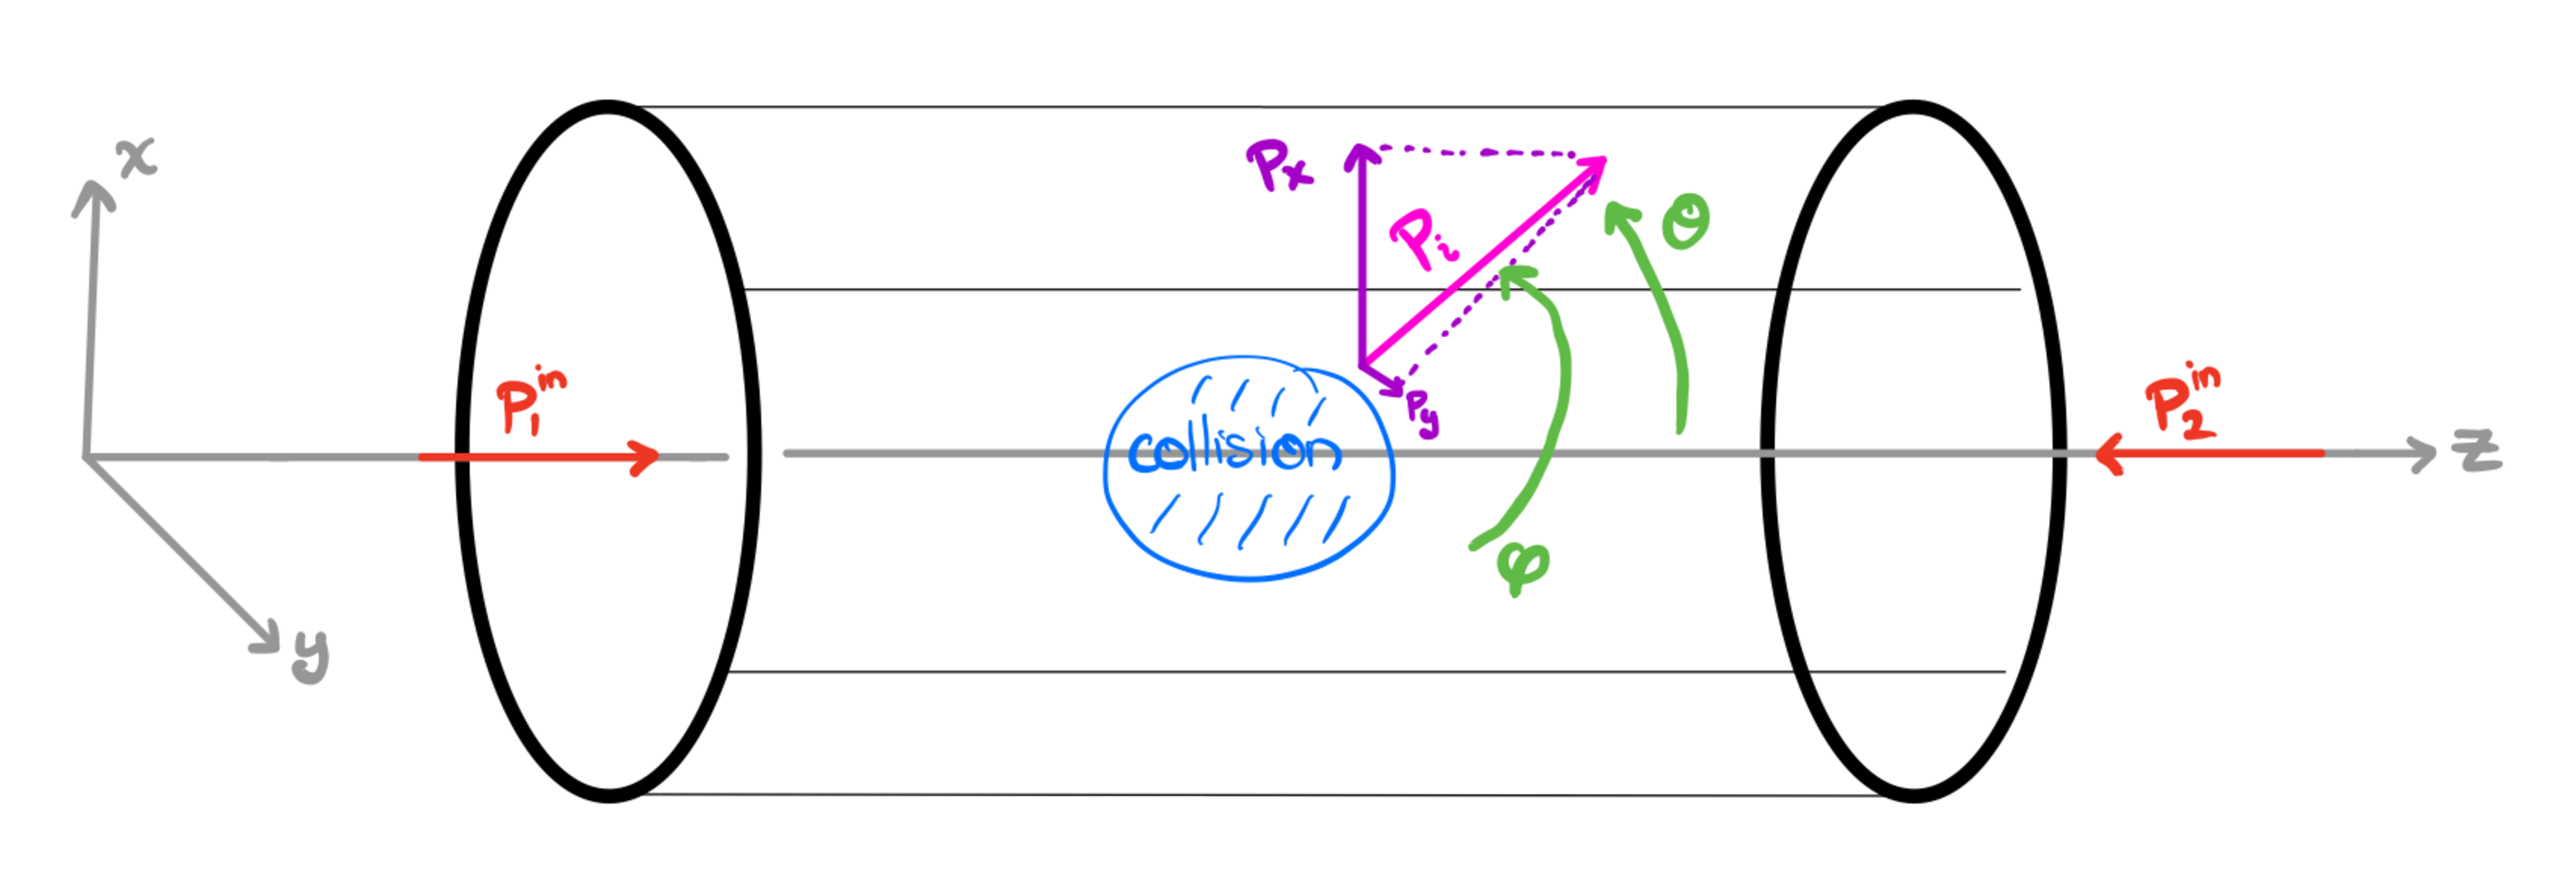
\includegraphics[width = 0.6\textwidth]{collider_kinematics}
	\caption{Kinematics of final-state momentum $\vec p$ in the center of mass frame. Note that $\phi$ is taken to be 0 on the $y$ axis instead of the $x$ axis as it's 
	technically defined, that's just an inconsistency in this drawing.}
	\label{fig:kinematics}
\end{figure}

The polar angle $\theta$ is often replaced with a coordinate $\eta$ called the \textbf{pseudorapidity}, which is defined as:
\begin{equation}
	\eta := \log\cot\frac{\theta}{2}\sim\frac{\pi}{2} - \theta + \mathcal O(\theta^2)
\end{equation}
where we have Taylor expanded $\eta$ for small values of $\theta$. This is a geometrical quantity which is typically used as a replacement for 
$\theta$ in collider data. If we consider the production of massless particles, $m_f = 0$, then the rapidity ends up precisely equalling the 
pseudorapidity. Nonetheless, the $\eta$ coordinate is used for all particles, despite the fact that it only has a clear kinematical interpretation 
for massless particles. $\eta$, as well as differences in $\eta$, is not a boost invariant when particles are not massless. 

We often abuse notation and define the \textbf{invariant mass} of a process:
\begin{equation}
	M^2 := \bigg|\sum_\textnormal{final states j} p_j^\mu\bigg|^2
\end{equation}
If the process features a parent decaying into daughters, this will give us the original mass of the parent particle, assuming all the daughters 
are measured. Furthermore, in a two particle collision this will equal the Mandelstam variable $s$. 
For a $1\rightarrow 2$ particle decay $A\rightarrow BC$ (this often happens in $W$ production and is how the mass of the W boson is 
measured) with final state transverse momenta $\vec p_T^{\;(1)}$ and $\vec p_T^{\;(2)}$, we define the \textbf{transverse energy} and 
\textbf{transverse mass} as:
\begin{align}
	E_T := \sqrt{M^2 + p_T^2} && m_T^2 := \left(E_T^{(1)} + E_T^{(2)}\right)^2 - \left(\vec p_T^{\;(1)} + \vec p_T^{\;(2)}\right)^2
\end{align}
where $M$ is the invariant mass of the process. If the final momenta are purely longitudinal ($\vec p_T^{\;(1)}$ and $\vec p_T^{\;(2)}$ are 0), 
then the transverse mass vanishes, and if the final momenta are purely transverse ($\vec p_T^{\;(1)} = \vec p^{\;(1)}$ and 
$\vec p^{\;(2)} = \vec p^{\;(2)}$) then the transverse mass equals the invariant mass. In any case, the transverse mass is always bounded by 
$0\leq m_T \leq m_A$, and when the bounds are saturated the daughters are either purely transverse or longitudinal. \textbf{The transverse 
mass is invariant upon boosting the parent particle $A$ along its collinear axis, and it is also not sensitive to transverse perturbations}: upon 
boosting $B$ or $C$ by a small parameter $\beta$ in the transverse plane, one can show that $m_T$ does not change at first order in 
$\beta$ and the first corrections are $m_T\mapsto m_T + \mathcal O(\beta^2)$. 

Let's turn our attention to what is actually measured at colliders. On paper, a collider event is completely defined by knowledge of the final 
state particles and their momenta; the final particle trajectories, once measured, can be extrapolated back to the collision point as long as 
their momenta are picked up in the detector. Since the detector is measuring final state particles at some length away from the collision point, 
it often happens that there are \textit{intermediate particles formed after the collision but before the final particles are picked up in the 
detector}. For example, in the Higgs discovery, the Higgs was created through gluon fusion and then decayed into two photons as 
$gg\rightarrow h\rightarrow\gamma\gamma$. When the LHC picked up this process, it did not measure the Higgs directly, but rather the two 
photons. Since they decayed from a real Higgs, their trajectories did not originate from the collision point, but rather from where the Higgs 
decayed. With complete knowledge of the final state momenta, we see that one can extrapolate what occurred to generate that final state, but 
it is by no means easy to establish this. 

Unfortunately, not all particles are picked up by detectors, and so complete knowledge of the final state is not always possible. Detectors are 
made to pick up energy deposits from a variety of particles, but the one type of particles that they will not pick up is \textbf{neutrinos}, since 
they are uncharged and don't interact with much. As such, we often measure the \textbf{missing transverse momentum / energy}
\begin{align}
	\slashed{\vec p_T} := - \sum_\textnormal{final states j} \vec p_T^{(j)} && \slashed{E_T} := |\slashed{\vec p_T}|
\end{align}
where the sum on $j$ picks up only the measured final states. Since $\sum \vec p_T = 0$ whens summing over all final states, $\slashed{\vec p_T}$ will give 
the sum of the transverse momenta of the final states which were not measured by the detector. For example in a $W^-\rightarrow e^-
\overline\nu_e$ decay, since there will be one missing particle (the neutrino), $\slashed{\vec p_T} = \vec p_T^{\;(\nu)}$ and we therefore know 
where the neutrino went after the collision. 

Detectors are typically made in layers, where each layer is able to track a particle with different hadronic or electronic 
properties~\cite{particle_detectors}. Once a detector triggers, as the particle passes through the different layers it deposits a different amount 
of energy in each layer it interacts with. There are three primary units which make up a detector; they are usually layered around the collision 
point in the following order, with the trackers being the innermost part and the muon detector being the outermost.
\begin{itemize}
	\item Trackers: Measures the momentum of charged particles.
	\item Calorimeters: Measures the energy of particles. Calorimeters can either be \textit{electric} or \textit{hadronic}: electric calorimeters 
	measure energies of photons and electrons, and hadronic calorimeters measure energies of hadrons. They are designed to stop any 
	particle other than a muon or a neutrino.
	\item Particle identifier: Identifies the type of particles which passes through based on determining what type of radiation the particle 
	emits.
	\item Muon detector: Muons don't interact very much with matter. They are very fast and require a lot of material to stop them, and 
	chambers to identify muons and track them usually make up the outer layer of most detectors. 
\end{itemize}

Particle detectors also have finite resolution: in general, particles need to travel far enough in the detector to be identified. The 
\textbf{spatial resolution} of a detector is how far apart two particles need to be for the detector to resolve them as distinct: typically this 
is on the order of 10 to 100 $\mu$m. Likewise, the \textbf{time resolution} of a detector is the amount of time required to resolve two 
distinct events, and is also the smallest amount of time a particle's lifetime (in the \textit{lab frame}; since particles are moving so fast there 
is usually significant time dilation between the rest frame lifetime $\tau$ and the lab frame lifetime $\gamma\tau$) must be to be picked up by 
the detector. In modern detectors, the time resolution is typically on the order of nanoseconds to microseconds.

% radiative return

\newpage
\section{Boson production at hadron colliders}

To estimate observables and cross sections from the LHC, we must start off by computing the inclusive\footnote{By inclusive, we mean 
$\sum_X\sigma(pp\rightarrow X)$, where $|X\rangle$ is any state that the proton collision can generate.} $pp$ scattering cross section. 
Unfortunately, this is not easy to do theoretically or experimentally, so we will provide a quick and dirty way to estimate the inclusive cross 
section. We know that $\sigma(n-U^{235})\approx 1\;\mathrm{bn}$ and the scattering cross section should roughly scale like the area of the 
nucleon. The volume of the nucleon is roughly proportional to the atomic number $Z$, so $r\sim Z^{1/3}$ and therefore $\mathrm{Area}
(p^+) / \mathrm{Area}(U^{235})\approx \left(\frac{1}{235}\right)^{2/3}\approx 0.03$. Thus we expect the $pp$ cross section to be about:
\begin{equation}
	\sigma(pp; \;\mathrm{inclusive})\approx 30 \;\mathrm{mbn}
\end{equation}
It turns out that this gives us a reasonably good estimate of the proton's total cross section. This is a good thing to keep in the back of your 
mind for LHC physics, because to get a relative cross section for a process one typically wants to look at $\sigma(pp\rightarrow X)$, 
normalized by $\sigma(pp;\;\mathrm{inclusive})$. This is also consistent with \textit{the proton's size being about a femtometer}. If we 
want $\sigma\sim\pi r_p^2$, then we see that:
\begin{equation}
	\sigma(pp; \;\mathrm{inclusive})\approx\pi r_p^2 \approx 3\times 10^{-30} \;\mathrm{m}^2 = 0.03 \;\mathrm{bn} = 30\;\mathrm{mbn}
\end{equation}

Suppose we wish to compute how frequently a $W$ boson is produced at the LHC. This will be (very) roughly on the order of the scale of the 
weak interactions, which is the Fermi coupling $G_F$. Naive dimensional analysis gives us a direct scaling with $G_F$, as both $\sigma$ and 
$G_F$ has mass dimension -2, so:
\begin{equation}
	\sigma(pp\rightarrow W)\sim G_F\approx 10^{-5}\textnormal{ GeV}^{-2}\sim 4\times 10^{-7}\textnormal{ fm}^2 = 4\times 10^{-9}\textnormal{ bn} \nonumber
\end{equation}
We thus see that $\sigma(pp\rightarrow W) / \sigma(pp; \textnormal{ inclusive})$ is roughly $10^{-7}$, so we can estimate that a $W$ boson will 
be produced at the LHC in about every $10^7$ proton collisions. 

\subsection{Z bosons and the Drell-Yan process}

Let's most towards something a little more quantitative: the \textbf{Drell-Yan process}. This process is very useful for our purposes for 
estimating cross sections, and is particularly useful in hadron-hadron colliders. The cross section is often used in computations to rigorously 
provide relations between partonic processes and hadronic processes, which is necessary when we're colliding hadrons together and want to 
compute cross sections with the parton model\footnote{If we were instead working in an electron-hadron collider like HERA, we'd want to use 
DIS instead of Drell-Yan because it is process specific.}. The Drell-Yan process is leption-antilepton pair production through mediator bosons, 
i.e. at the LHC it is 
\begin{equation}
	HH\rightarrow (\gamma\textnormal{ or } Z) \rightarrow \ell\overline\ell
\end{equation}
where $H$ is a hadron. The important point regarding Drell-Yan is that the process \textbf{factorizes} in the parton model just like DIS, so that we can write the total 
hadronic cross section as an integral with the appropriate PDF insertions:
\begin{equation}
	\frac{d\sigma}{d m^2} = \int dx_1\,dx_2\, f_q(x_1, \mu) f_{\overline q}(x_2, \mu) \frac{d\hat\sigma(q\overline q\rightarrow \ell\overline\ell, \mu)}{dm^2} + (q\leftrightarrow\overline q)
\end{equation}
where $m^2 = \hat s$ is the invariant mass. The total $d\sigma / dm^2$ is what would be shown in data at the LHC, so the parton model 
allows us to relate this to things we can easily compute from the Standard Model. Since the partonic momenta $p_1, p_2$ are related to the 
hadronic momenta $P_1, P_2$ by $p_i = x_i P_i$, we see that $\hat s = (p_1 + p_2)^2 = 2 p_1\cdot p_2 = 2 x_1 x_2 P_1\cdot P_2 = x_1 x_2 
S$, where $\sqrt S = 13$ TeV is the CoM energy of the colliding hadrons (this is all assuming the particles have sufficiently small mass $<< \sqrt S$). 
We can therefore explicitly write the factorization as a multiplication of a partonic cross section with a so-called \textbf{luminosity function} 
$\mathcal L_{q\overline q}$:
\begin{align}
	\frac{d\sigma}{dm^2} = \mathcal L_{q\overline q}(m^2) \frac{d\hat\sigma}{d\hat s} && \mathcal L_{q\overline q}(\hat s) = \int dx_1\,dx_2\, f_q(x_1, \mu) f_{\overline q}(x_2, \mu) 
	\delta(x_1 x_2\hat s - S)
\end{align}

Assuming factorization, we can compute this at the partonic level.
This decay occurs at tree level through an $s$-channel exchange of the mediator boson: it also equals the DIS diagram flipped at a 90 degree angle.
\begin{equation}
	i\hat{\mathcal M} = \begin{gathered}
	\feynmandiagram [horizontal=a to b] {
	  i1 [particle=\(q\)] -- [fermion, edge label'=\(p_1\)] a -- [fermion, edge label'=\(p_2\)] i2 [particle=\(\overline{q}\)],
	  a -- [photon, edge label=\(\gamma / Z\), momentum'=\(q\)] b,
	  f1 [particle=\(\ell\)] -- [anti fermion, edge label'=\(k_1\)] b -- [anti fermion, edge label'=\(k_2\)] f2 [particle=\(\overline{\ell}\)],
	};
	\end{gathered}
	= \frac{1}{\hat{s}} \left(\overline u(k_1) \Lambda_\ell^\mu v(k_2)\right) \left(\overline v(p_2) \Lambda_{q, \mu} u(p_1)\right)
\end{equation}
Hats will be used to denote partonic observables, as in this diagram where we are specifically computing a partonic process. $\hat s$ is the partonic center of mass energy, 
$\hat s = (p_1 + p_2)^2 = q^2$. The $\Lambda$ piece depends on the coupling and can be read off from the SM Lagrangian as one of the following terms, depending 
on if we are working with $\gamma$ or $Z$ exchange:
\begin{equation}
	\Lambda_f^\mu := \begin{cases}
		g_Z (g_V^{(f)} \gamma^\mu + g_A^{(f)}\gamma^\mu\gamma_5) & \textnormal{Z exchange} \\
		 e Q_f \gamma^\mu & \gamma\textnormal{ exchange}
	\end{cases} \nonumber
\end{equation}
where $g_Z := \frac{g}{\cos\theta_w} = \frac{e}{\sin\theta_w\cos\theta_w}$ is the strength of the $Z$ coupling.

Let's simplify to the case of $Z$ exchange. After resumming $Z$ loops, the partonic cross section takes the form of a \textbf{Breit-Wigner 
distribution}:
\begin{equation}
	\frac{d\hat\sigma(q\overline q\rightarrow Z\rightarrow\ell\overline\ell)}{d\hat s} \approx \frac{g_Z^4}{(\hat s - m_Z^2)^2 + \Gamma_Z^2 m_Z^2}
\end{equation}
The width of the Z boson is about $\Gamma_Z\sim g_Z^2$, and is measured to be $\Gamma_Z = 2.5$ GeV. Note that since $\Gamma_Z\sim 
g_Z^2$, near resonance ($\hat s = m_Z^2$) the cross section goes as $d\hat\sigma\sim g^2$, and off resonance it goes as $d\hat\sigma\sim 
g_Z^4$: resonance enhances $\hat\sigma$ by a factor of $1 / g_Z^2$, which in the weak coupling limit is quite a large enhancement. 
Since the Breit-Wigner distribution is peaked around $m_Z$ with a width of $\Gamma_Z$, as we take $\Gamma_Z / m_Z << 1$ the 
distribution becomes a narrow peak and in fact approaches a $\delta$ function. This is called the \textbf{narrow width approximation}:
\begin{align}
	\frac{d\hat\sigma}{d\hat s}\approx \frac{g_Z^4\pi}{\Gamma_Z m_Z} \delta(\hat s - m_Z^2)
\end{align}
The dimensions on this are consistent, because $[\delta(\hat s)] = - [\hat s] = -2$. The narrow width approximation puts the intermediate $Z$ 
boson on its mass shell, so the total cross section then factorizes as a branching ratio:
\begin{align}
	\hat\sigma(q\overline q\rightarrow Z \rightarrow\ell\overline\ell) &= \hat\sigma(q\overline q\rightarrow Z)\mathrm{BR}(Z\rightarrow\ell\overline\ell)\nonumber \\
	\mathrm{BR}(Z\rightarrow\ell\overline\ell) &:= \frac{\Gamma(Z\rightarrow\ell\overline\ell)}{\Gamma_Z}
\end{align}
For $\ell = e^-$, this branching ratio is about BR$(Z\rightarrow e^- e^+) \approx 0.03$. 

The cross section for $p\overline p\rightarrow\ell\overline\ell + X$ has been measured at $p\overline p$ colliders (note the LHC is primarily a 
$pp$ collider) and is plotted in Figure~\ref{fig:lepton_production_drell_yan}.Note that we have only discussed the $Z$ contribution to this 
cross section, but the photon contribution should also be included. It scales as $1 / \hat s$ as well and is more dominant at low energies, but 
has no resonance peak since the photon is massless. 
\begin{figure}[H]
	\centering
	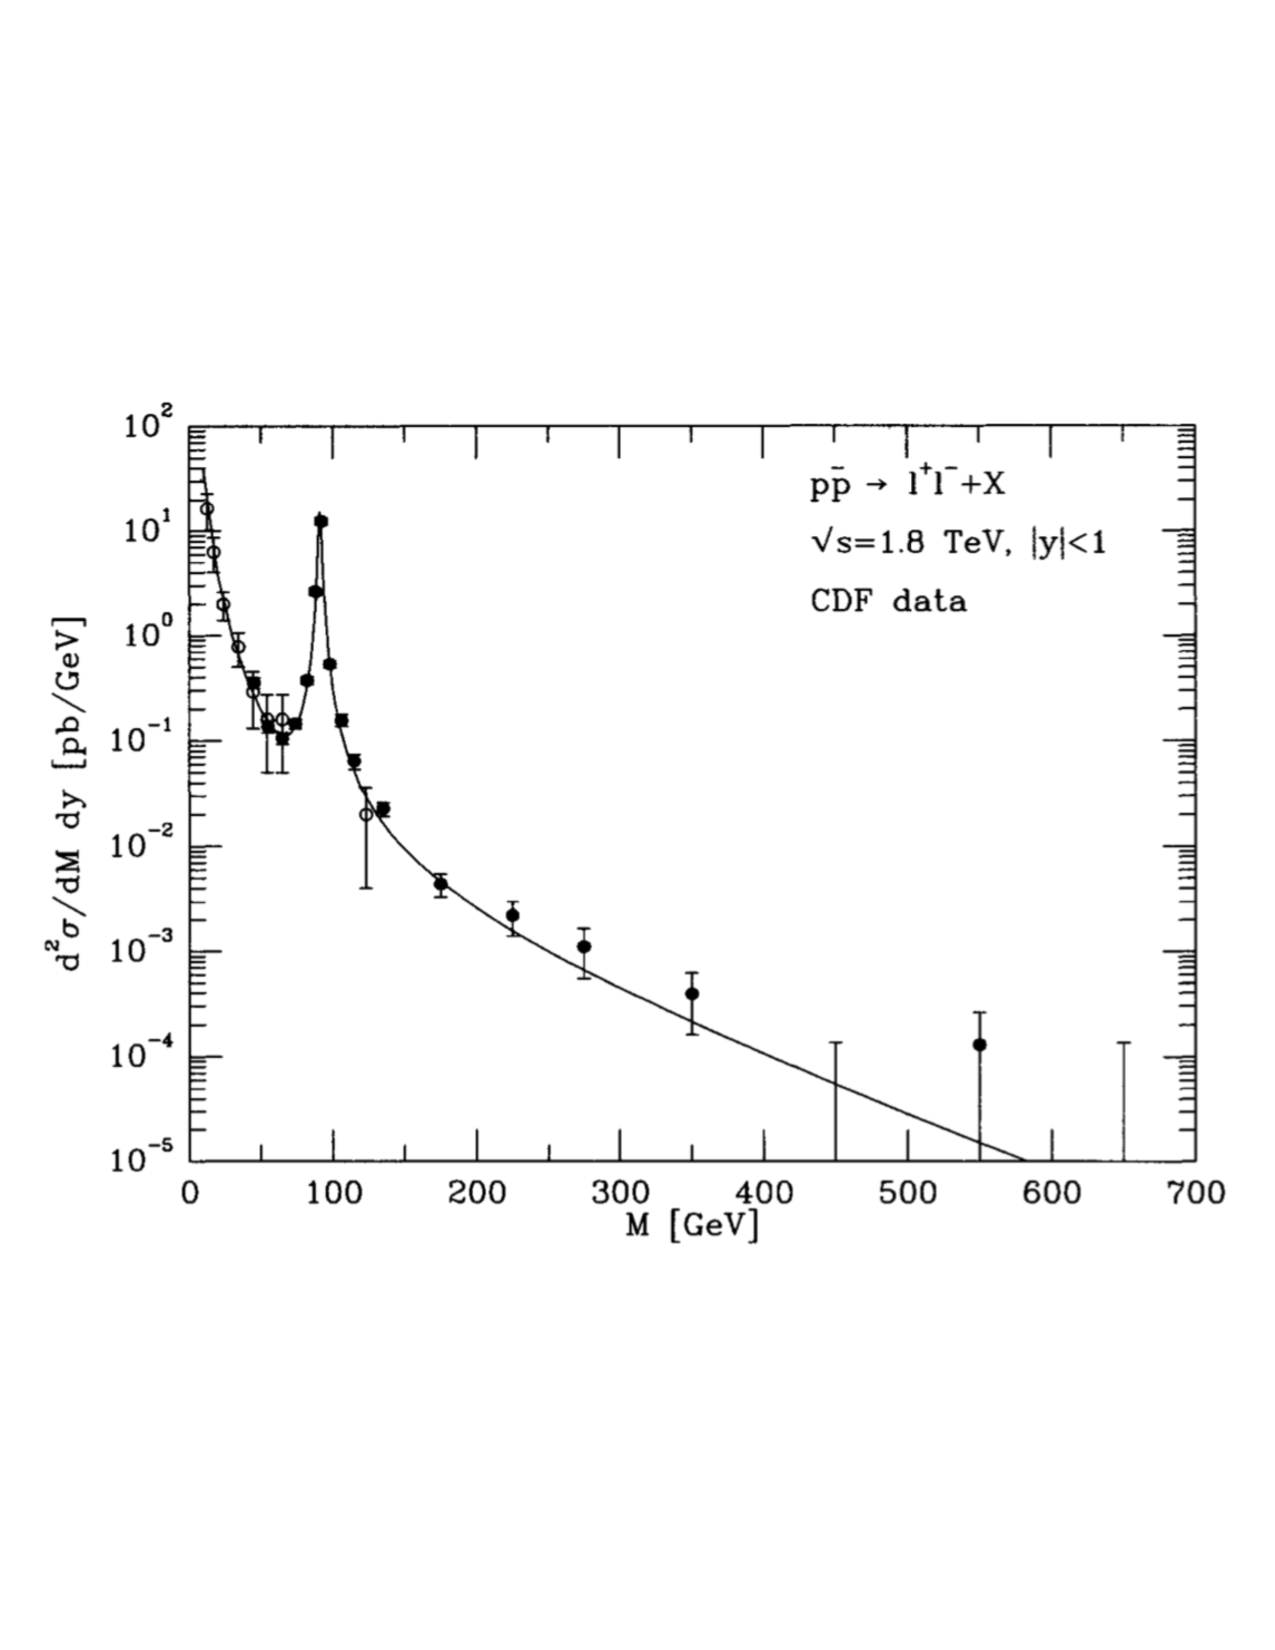
\includegraphics[width = .6\textwidth]{lepton_production_drell_yan}
	\caption{Differential cross section for $p\overline p\rightarrow\ell\overline\ell + X$ at a $p\overline p$ collider~\cite{ellis}. 
	Theoretical predictions at NLO are plotted against the data as the black line. One can clearly see the resonance at $M = m_Z = 91$ GeV, 
	which is due to the Breit-Wigner form of the distribution. Note that from this plot one can directly measure the mass of the $Z$ boson by 
	fitting the resonance peak to the theoretical predictions.}~
	\label{fig:lepton_production_drell_yan}
\end{figure}

\subsection{Production of $W^\pm$ bosons}

Let's consider the other massive vector boson in the Standard Model: the $W$ boson. $W$ bosons can also be produced at hadronic 
colliders, but not directly through the Drell-Yan process as they only couple together different types of fermions. Instead, the mass of the 
$W$ is typically measured via the decay $W\rightarrow e^-\overline\nu_e$. Unfortunately in this case, there are additional complications 
because the neutrino is not measured by the detector. This provides an excuse to show where the transverse mass is applicable at 
particle colliders. 

To study lepton production through the $W$ at hadron colliders, we consider the process $q_i\overline q_j\rightarrow W^\pm\rightarrow 
\ell^\pm\nu_\ell$, where the neutrino is either $\nu$ or $\overline\nu$ to conserve lepton number. Since we can only meaasure $\ell$ 
production, we must write our predictions in terms of the kinematical variables of the lepton. Let $\theta^*$ be the polar angle of the lepton 
in the $W$ rest frame (where the $z$ axis is oriented along the $W$'s direction of motion. Then one can show that:
\begin{equation}
	\frac{1}{\hat\sigma}\frac{\hat\sigma(q\overline q\rightarrow W\rightarrow \ell\nu)}{d\cos\theta^*} = \frac{3}{8} (1 + \cos^2\theta^*)
	\label{eq:w_production_theta}
\end{equation}

The immediate issue with this equation is that the $W$ rest frame is not known, since we don't know the neutrino's momentum. If we could 
measure $\vec p^{(\nu)}$, then we would immediately know the 
\begingroup
\begin{wrapfigure}{r}{.3\textwidth}
	\vspace*{-.5cm}
	\centering
	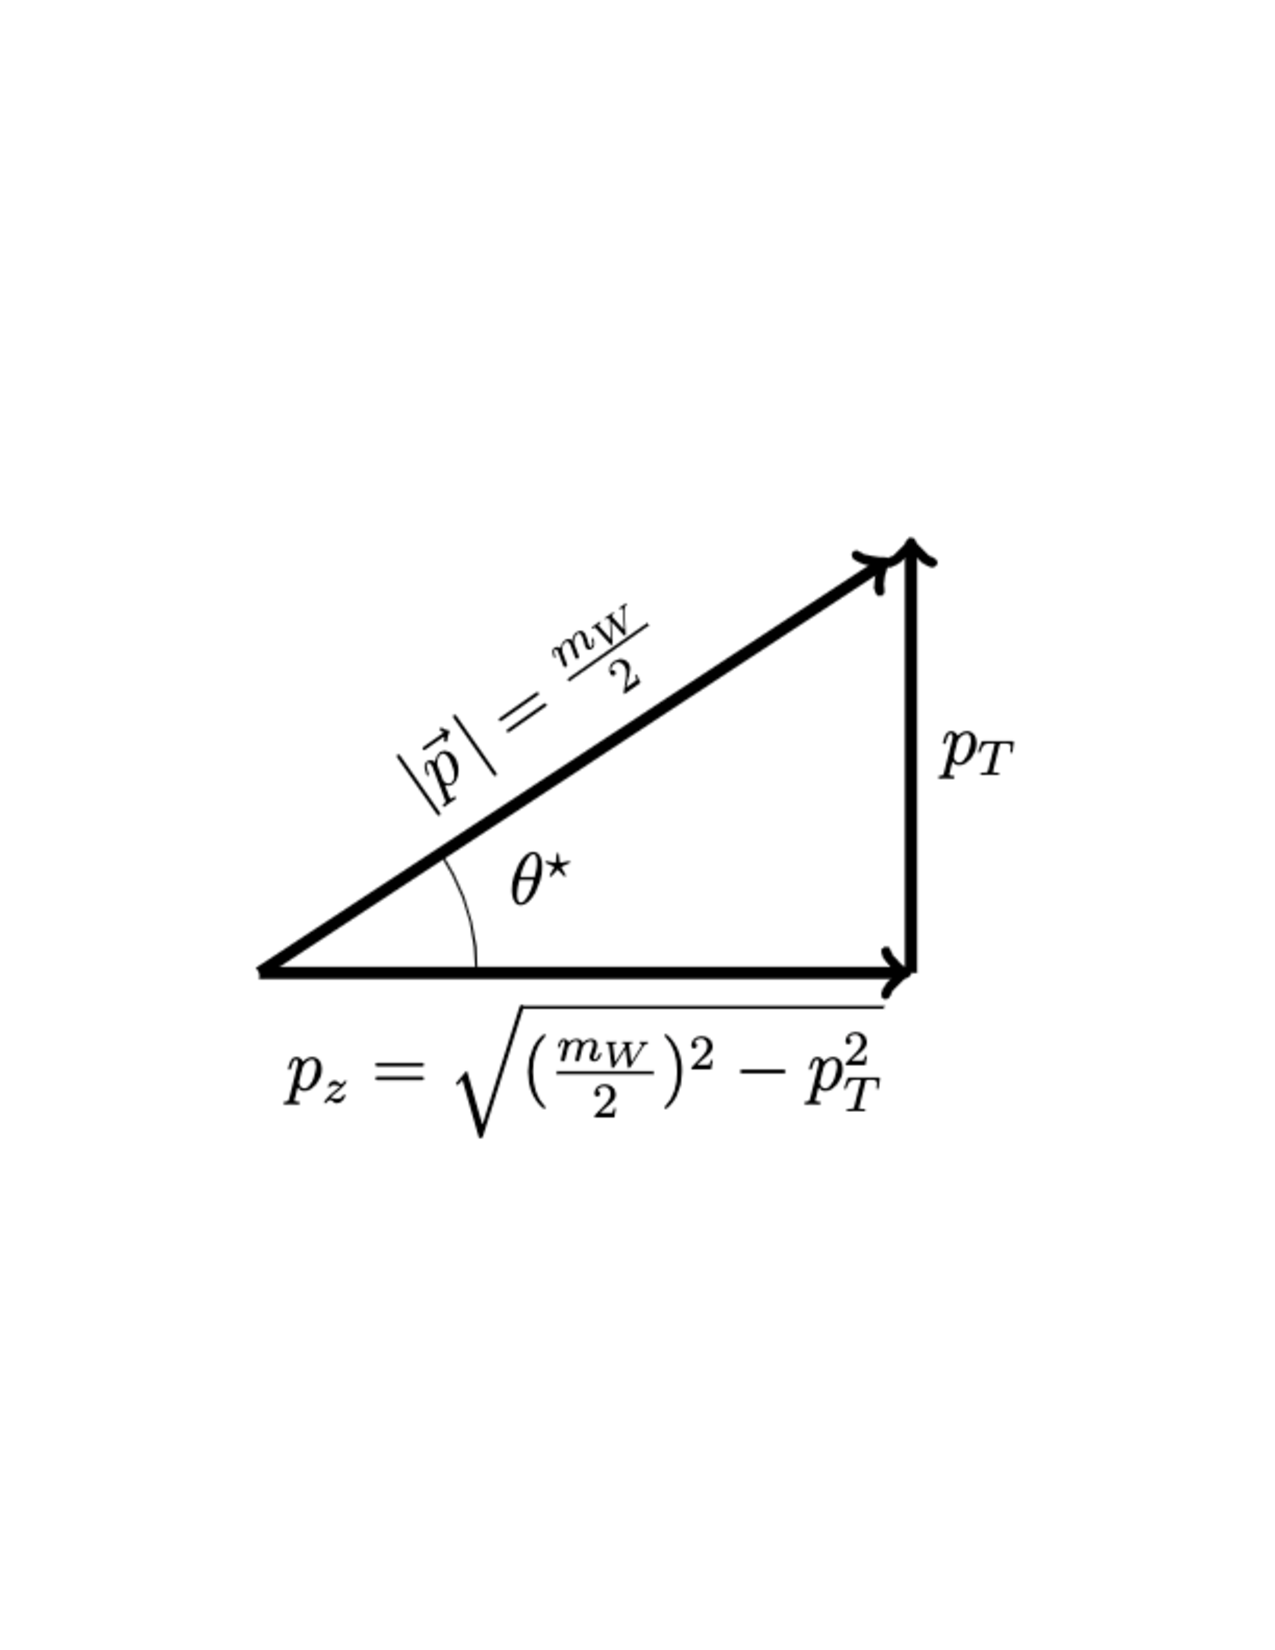
\includegraphics[width = .25\textwidth]{w_production_triangle}
	\caption{Lepton kinematics.}
	\label{fig:w_triangle}
\end{wrapfigure}
$W$ rest frame by taking the frame where $\vec p^{(\nu)} = -\vec p^{(\ell)}$, but unfortunately we don't have that information. 
However, what we can do instead is use our knowledge of the $W$ mass $m_W$ to tell us where the rest frame should be. 
In the $W$ rest frame (assuming $\ell$ is massless), $p^{(\ell)}_\mu = (\frac{1}{2} m_W, \vec p)$ and $p^{(\nu)}_\mu = (\frac{1}{2} m_W, 
-\vec p)$. Writing this out in terms of the transverse momentum $\vec p^{(\ell)} = (\vec p_T, p_z)$, we arrive at the triangle in 
Figure~\ref{fig:w_triangle}. It is then immediate that $\cos\theta^* = \sqrt{1 - 4 p_T^2 / m_W^2}$, and we can change the variables in 
Eq.~(\ref{eq:w_production_theta}) to rewrite the cross section in terms of $p_T$ and $m_W$ instead of $\theta^*$. 

\endgroup
Swapping out $\theta^*$ for $p_T$ and This change of variables gives us the following result for the cross section:
\begin{equation}
	\frac{1}{\hat\sigma}\frac{d\hat\sigma}{d p_T} = \left(\frac{3}{m_W^2} \frac{p_T}{\sqrt{1 - 4 p_T^2 / m_W^2}}\right) \left(1 - 
	\frac{2 p_T^2}{m_W^2}\right)
	\label{eq:W_pT_sigma}
\end{equation}
The singularity in the first term of this expression gives rise to what is called the \textbf{Jacobian peak} at $p_T = \frac{m_W}{2}$ in the $W$ 
production data. When higher order production effects are included, it smooths out the singularity but still preserves the location of the 
maximum. Historically, measurement of this peak was the first way that the mass of the $W$ boson was measured. It is the result 
of changing variables on the derivative $d / d\cos\theta^*$. The second term in parentheses is the $1 + \cos^2\theta^*$ term written out in 
these new variables. 

One can also change variables from $p_T$ to instead measure the cross section as a distribution over the transverse mass $m_T$ 
instead of the transverse momentum $p_T$. Since the transverse mass and transverse momentum are boost invariants, we can change 
variables in the center of mass frame, where $m_T = 2 p_T$. This variable transformation does not change Eq.~(\ref{eq:W_pT_sigma}) 
significantly, except it \textit{shifts the location of the Jacobian peak to $m_T = m_W$}:
\begin{equation}
	\frac{1}{\hat\sigma}\frac{d\hat\sigma}{d m_T^2} = \frac{3}{16 m_W^2}\frac{1}{\sqrt{1 - \frac{m_T^2}{m_W^2}}}\left(2 - \frac{m_T^2}{m_W^2}\right)
\end{equation}

Experimental data from the Tevatron collider which provided an early measurement of the $W$ mass is shown in Figure~\ref{fig:w_mass}. 
In it, one can clearly see the Jacobian peak at $m_T = m_W$. Note that although the cross section has a kinematic endpoint at $m_T = 
m_W$ and should not be defined for $m_T > m_W$, the measured distribution has a tail above the peak. This can be explained by a few 
reasons: 
\begin{enumerate}
	\item We only computed the cross section at tree level; higher order effects augment this process and do not have this singularity, and 
	the total cross section we see includes all orders of such effects.
	\item The $W$ boson has finite width, so it should be smeared out at the Jacobian peak.
	\item The $W$ boson may have a small nonzero transverse momentum which is not accounted for experimentally.
	\item The detector has finite resolution, so any experimental measurement will have additional uncertainties.
\end{enumerate}

\begin{figure}[H]
	\centering
	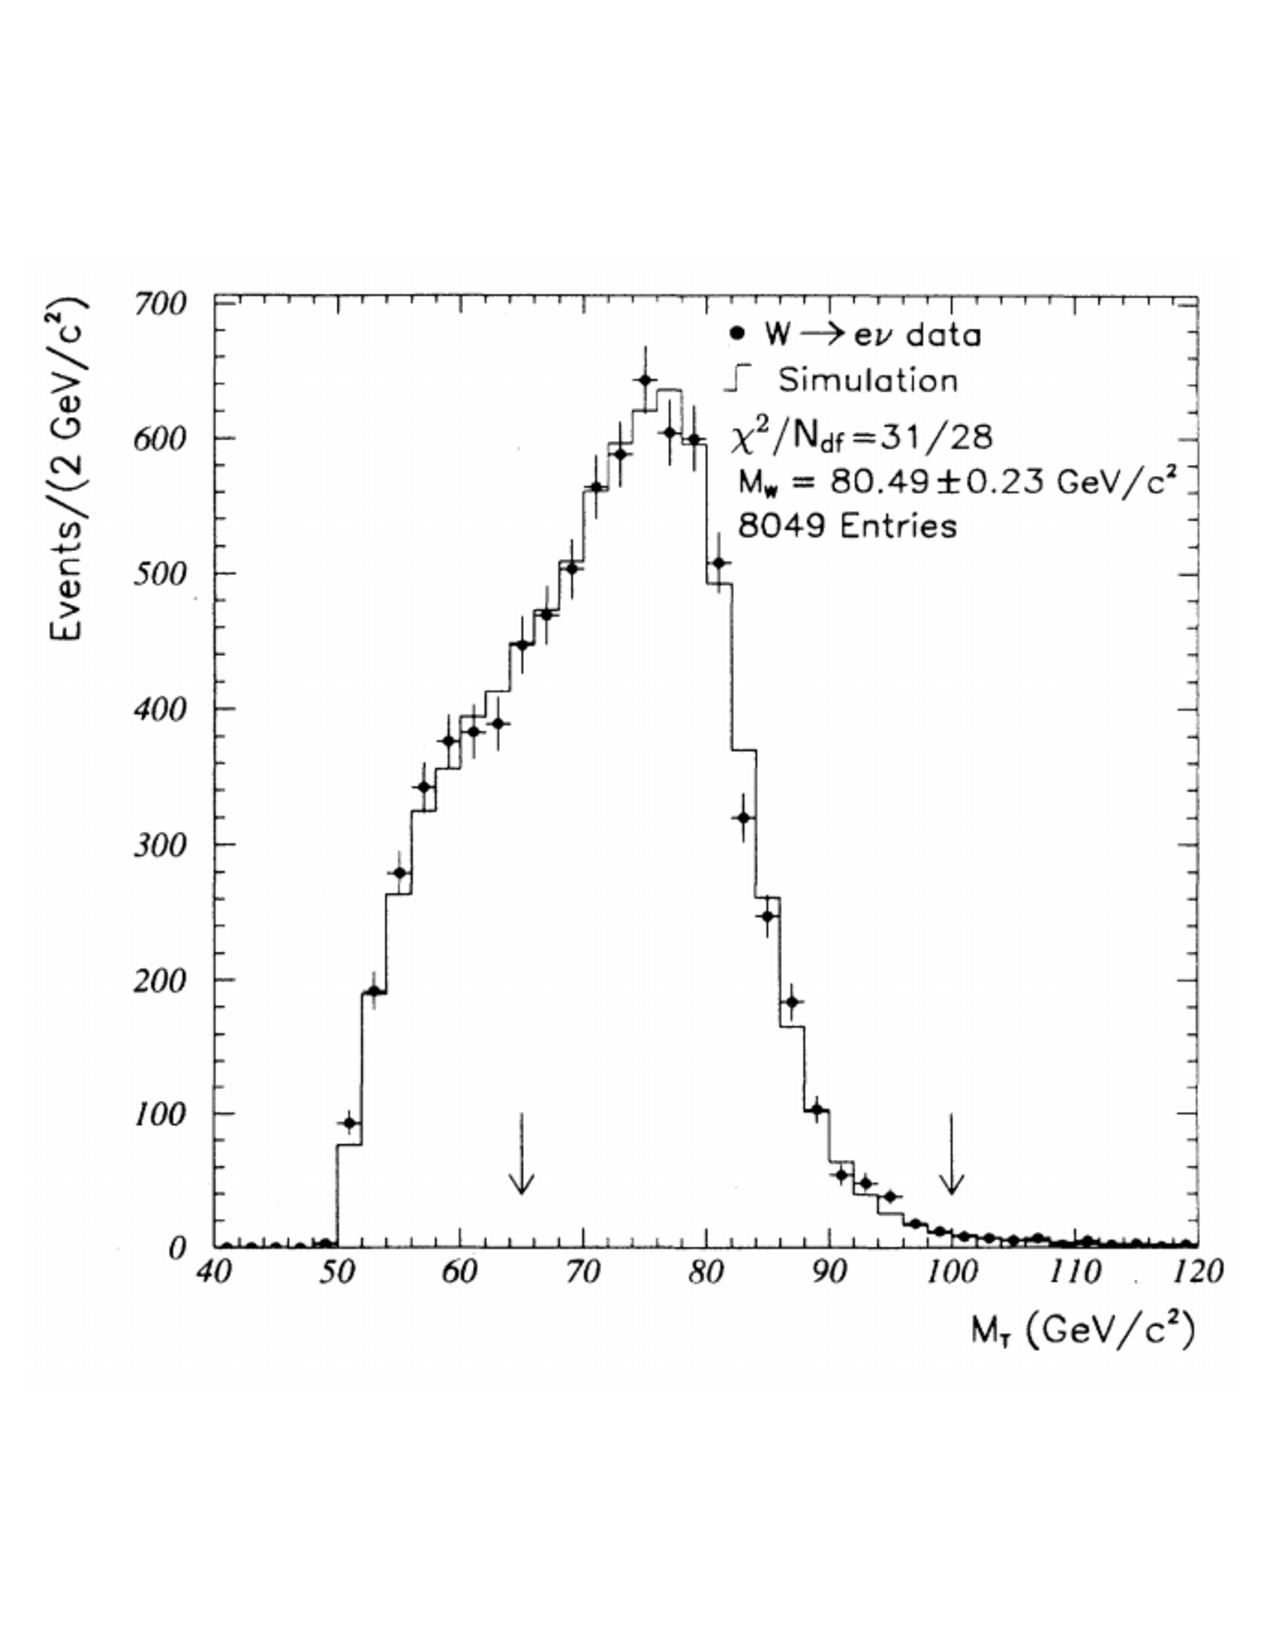
\includegraphics[width = 0.5\textwidth]{w_boson_mass}
	\caption{Measurement of the $W$ mass via the procedure described~\cite{w_mass}. This data is specifically for the process 
	$q\overline q\rightarrow W\rightarrow e\nu$, although we've discussed generalized this discussion to any lepton decay. The 
	analysis holds for each lepton in the massless limit, so naturally the cleanest data comes from the electron, as it is the lightest 
	lepton. }
	\label{fig:w_mass}
\end{figure}

\subsection{Vector boson generalities}

To summarize, up until now we've discussed how the vector boson masses can be measured at hadron colliders. The $Z$ boson mass can 
be seen through analyzing the Drell-Yan process, and its mass can be seen in the data as the resonance in the Breit-Wigner distribution. 
The $W$ boson requires a more complicated analysis because the final state neutrino is not measured, so we had to be more careful 
about the kinematics to compute the result from measured data at colliders, and we could not just look at the invariant mass of the 
entire process like we did with the $Z$ boson. 

One can also ask why we only look at leptonic final states to measure the resonance peaks, especially in the case of the $W$ boson where 
if we measured $W\rightarrow\mathrm{quarks}$, we could explicitly measure the kinematics of both outgoing particles since they would 
be electrically charged. This is because leptonic channels tend to be much cleaner than hadronic channels, since hadronic channels 
tend to produce \textbf{jets} instead of single-particle final states. Jets are directed clusters of hadrons which are formed from confinement: 
since final state quarks produced in processes cannot be free, these quarks must \textbf{hadronize} after the collision occurs, and this 
results in a large spray of hadrons in specific directions. The jets that are seen can be analyzed, but in general it is much more complicated to 
study decays to jets than leptonic process where we can see each lepton directly. 

Another observable that is often measured in the production of vector bosons at colliders is the asymmetry of $W$ production, which 
is related to the fact that $W$ bosons decay into different flavors of quarks. For example, consider $W$ production at a $p\overline p$ collider. 
The $W$ boson will not be produced isotropically because the quark PDFs in a proton / antiproton are not the same. If we only look 
at the valence quark contribution to $W^+$ production, we see that the $u$ quark in the proton and the $\overline d$ quark in the 
antiproton will interact to generate the $W^+$. However, the PDF $u(x)$ in the proton is larger than the PDF $\overline d(x)$ in the 
antiproton, as seen in Figure~\ref{subfig:proton_pdfs}. This means that on average, the forward-moving up quark will have more momentum 
than the backward moving $\overline d$ quark, and the $W^+$ will typically be produced in the direction of the proton. Likewise, the $W^-$ 
quark will be produced more often in the direction of the antiproton. The measure of this is called the \textbf{forward-backward asymmetry}, 
which is the observable:
\begin{equation}
	A_\mathrm{FB}(y) := \frac{d\sigma(W^+) / dy - d\sigma(W^-) / dy}{d\sigma(W^+) / dy + d\sigma(W^-) / dy}
\end{equation}
where $y$ is the pseudorapidity (recall that $y = 0$ corresponds to $\theta = \frac{\pi}{2}$, and here $y > 0$ is taken to be the direction of the 
incoming proton). These differential cross sections are plotted in Figure~\ref{subfig:fb_asymmetry} as a function of 
$y$. We see that $W^+$ boson production is peaked at positive $y$ (more $W^+$ is produced in the direction of the proton) and likewise 
the $W^-$ is peaked at negative $y$. 
\begin{figure}[H]
	\centering
	\begin{subfigure}[t]{.45\textwidth}
		\centering
		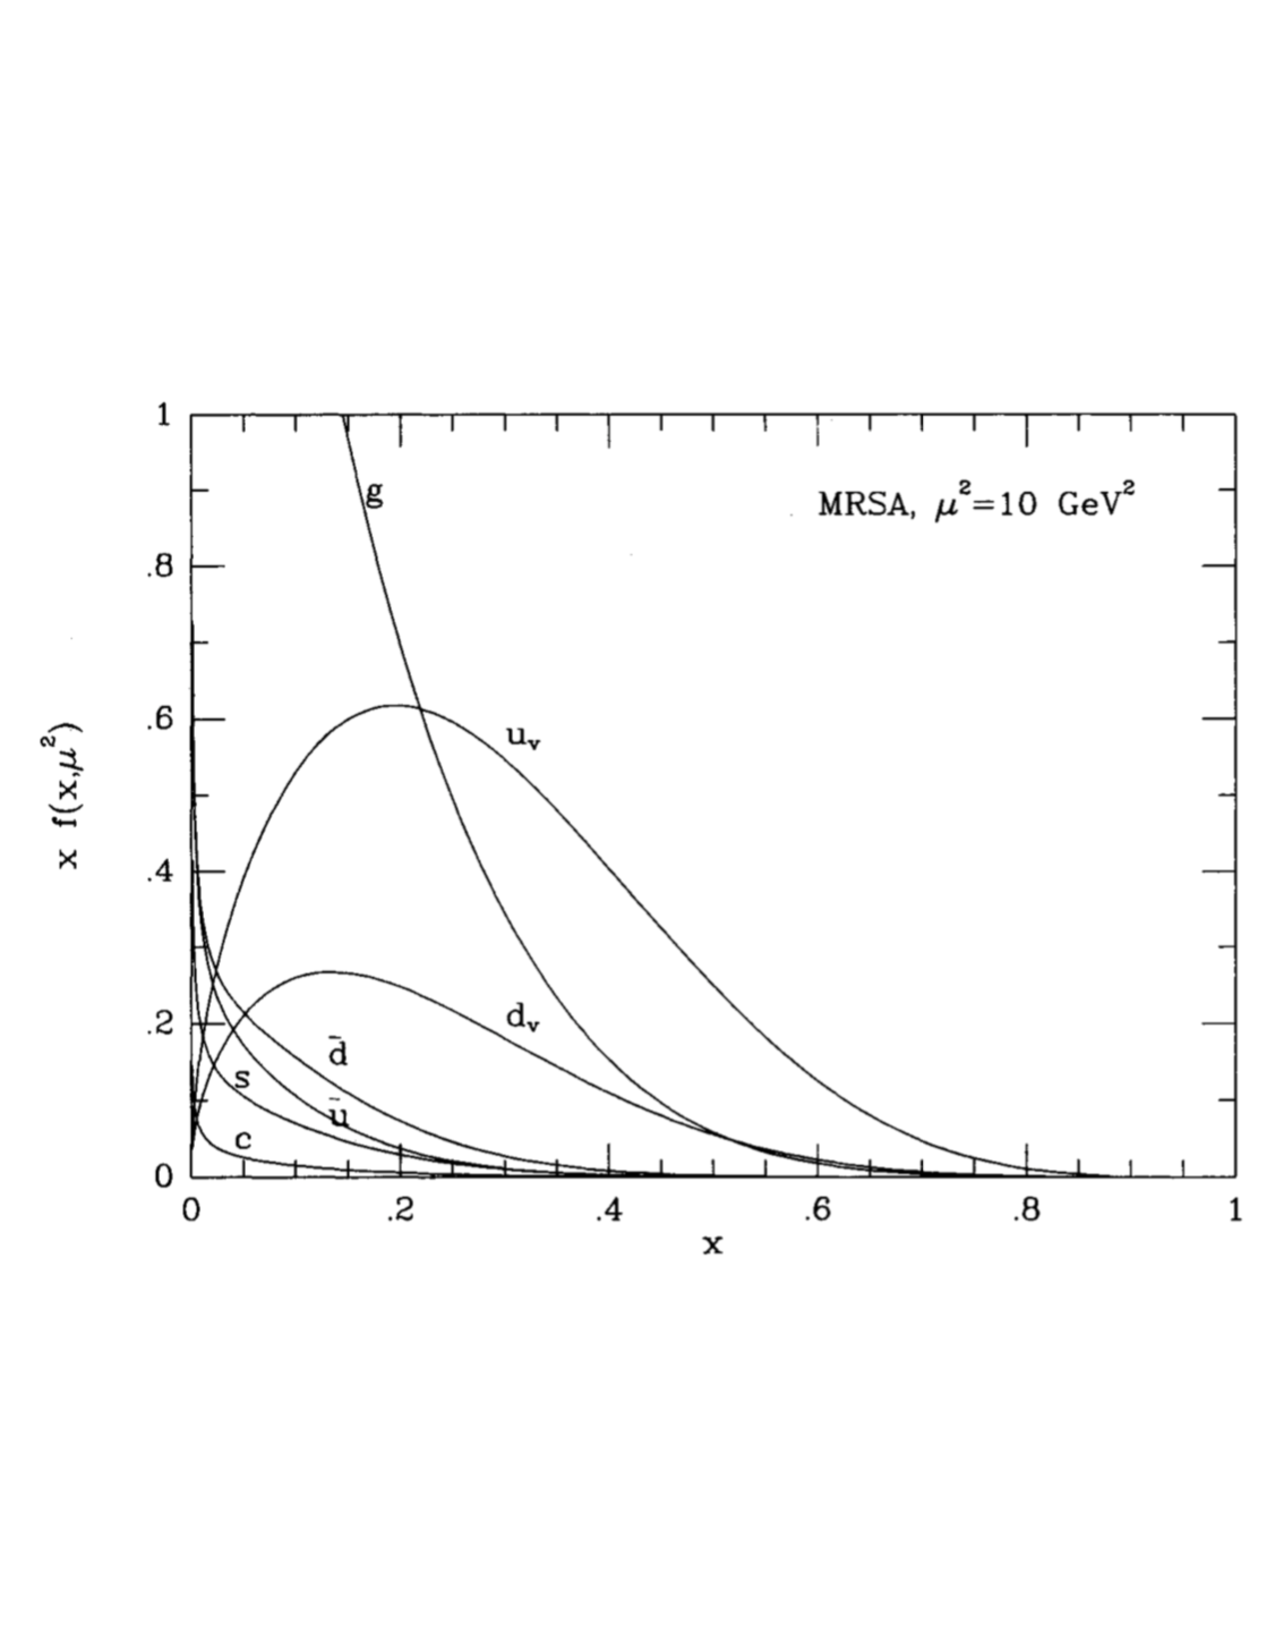
\includegraphics[width = \textwidth]{proton_pdfs}
		\caption{Quark and gluon PDFs in the proton.}
		\label{subfig:proton_pdfs}
	\end{subfigure}
	~
	\begin{subfigure}[t]{.45\textwidth}
		\centering
		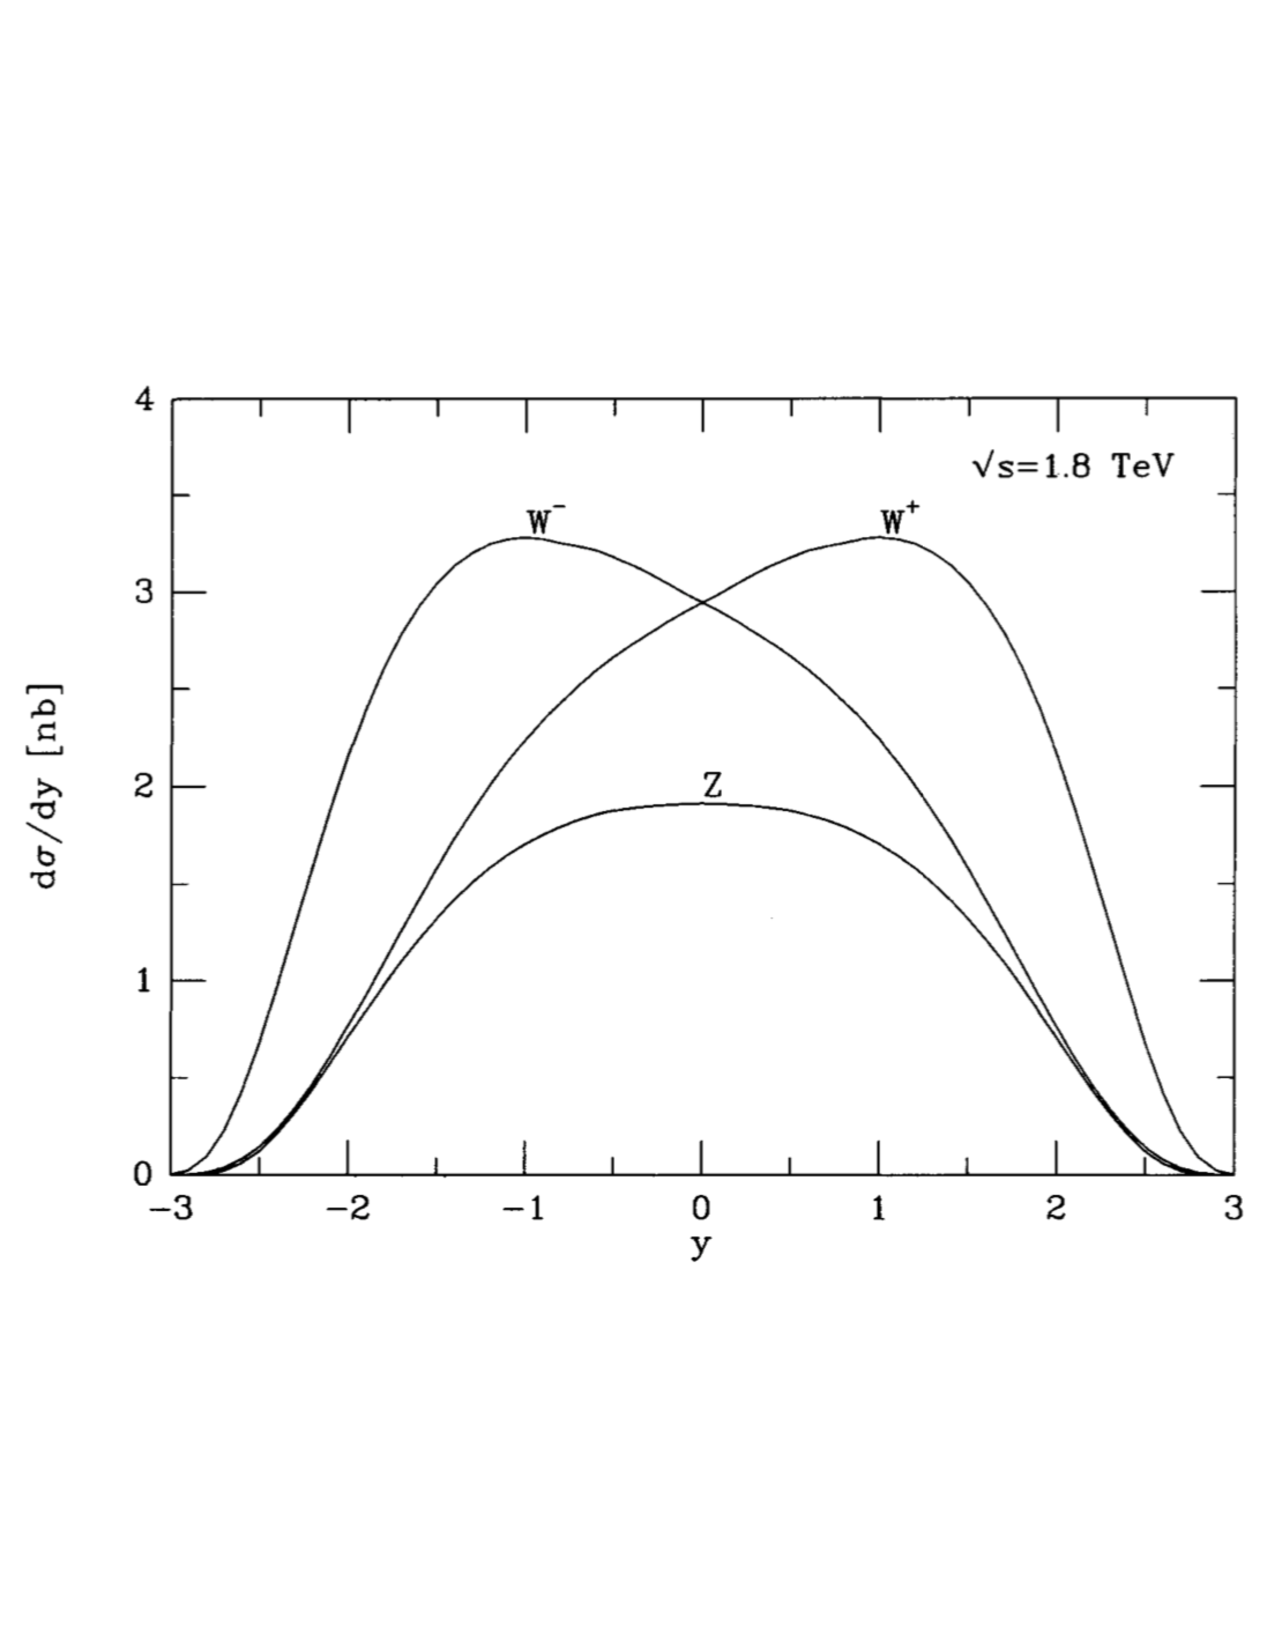
\includegraphics[width = \textwidth]{fb_asymmetry}
		\caption{$W$ and $Z$ distributions in $p\overline p$ collisions.}
		\label{subfig:fb_asymmetry}
	\end{subfigure}
	\caption{Relevant plots to $p\overline p\rightarrow W$ forward-backward asymmetry.~\cite{ellis}}
\end{figure}

We will end this section with some numerical values relevant for vector boson decays. The mass and width of the $W$ and $Z$ bosons 
can be found at the Particle Data Group's website\footnote{https://pdg.lbl.gov/2019/tables/rpp2019-sum-gauge-higgs-bosons.pdf}, and 
we will record them in Table~\ref{table:vector_boson_params}. Note that the $Z$ boson's width and mass are known to more precision 
than the $W$'s; that is because it is easier to measure, as we described above. I will record these in the Appendix as well with less 
significant figures, as we'll only need approximate masses for the Part III exam.
\begin{table}[H]
	\centering
	\begin{tabular}{ | c | c | c | }
		\hline
		Vector boson $V$ & Mass $m_V$ (GeV) & Width $\Gamma_V$ (GeV) \\
		\hline
		$W^\pm$ & 80.385(15) & 2.085(42) \\
		\hline
		Z & 91.1876(21) & 2.4952(23) \\
		\hline
	\end{tabular}
	\caption{Masses and widths of vector bosons.~\cite{pdg}}
	\label{table:vector_boson_params}
\end{table}

Let's also very briefly go over $W$ and $Z$ decays. The $W$ decays primarily two ways: to hadrons (which will form jets) or to leptons. 
The $W$ couples to fermions as (assuming no neutrino masses, i.e. no PMNS matrix):
\begin{equation}
	\mathcal L_{SM}\supset \frac{g}{\sqrt 2}\left(\overline u^i V_\mathrm{CKM}^{ij}\slashed{W^+} P_L d^j + \overline\nu_e \slashed W^+ P_L e + (e\leftrightarrow\mu) + (e\leftrightarrow\tau)\right) + \mathrm{h.c.}
\end{equation}
The $W$ thus has 9 possible decay modes into quarks at tree level. For the decay $W^+\rightarrow u^i\overline d^j$, the matrix element 
will contain a factor of the CKM matrix, $\mathcal M^{ij} = V_\mathrm{CKM}^{ij}(\mathrm{stuff})$, so the resulting cross section for 
$W^+\rightarrow u^i \overline d^j$ will contain a factor of $|V_\mathrm{CKM}^{ij}|^2$. We can use Wenzer's trick of CKM suppression to 
determine the dominant decay modes with the Wolfenstein parameterization of the CKM matrix (where $\lambda\approx 0.22$):
\begin{equation}
	V_\mathrm{CKM} = \begin{pmatrix} 1 - \frac{\lambda^2}{2} & \lambda & \lambda^3 \\
	-\lambda & 1 - \frac{\lambda^2}{2} & \lambda^2 \\
	\lambda^3 & \lambda^2 & 1
	\end{pmatrix}
\end{equation}
It is thus obvious that the off-diagonal hadronic decay modes will be suppressed by a factor of $\lambda$, $\lambda^2$, or $\lambda^3$, and 
therefore the primary decay modes will be to either $u\overline d$, $c\overline s$, or $t\overline b$. However, the top quark is heavier than 
the $W$, so only the first two decay modes are allowed. Therefore, the primary hadronic decays of the $W^+$ are $W^+\rightarrow d
\overline d$ and $W^+\rightarrow c\overline s$. 

Leptonic decay for the $W$ is easier: there are three decay modes (into $\ell^+\nu_\ell$ for any of the three leptons), and all the decay 
products are lighter than the $W^+$, so they are all kinematically allowed. Therefore, there are five possible decay products of the $W$. 
If we include color, we can put an estimate on the branching ratios $\mathrm{BR}(W^+\rightarrow f\overline f')$ by seeing how many decay 
modes are allowed for each particle. The quarks each come in 3 colors, and since each must be produced in a colorless combination, 
this gives 3 modes for each quark pair. The color quantum number does not exist for leptons, and so the total number of decay modes is 
9: 3 for $u\overline d$, 3 for $c\overline s$, and 1 for each lepton pair. So, we see the W should decay into jets about 2/3 of the time 
and each type of lepton about 1/9 of the time, which agrees well with experiment.
\begin{table}[H]
	\centering
	\begin{tabular}{ | c | c | c | c | c | c | }
		\hline
		$W^+$ decay mode & $u\overline d$ (jets) & $c\overline s$ (jets) & $e^+\overline\nu_e$ & $\mu^+\overline\nu_\mu$ & 
		$\tau^+\overline\nu_\tau$ \\
		\hline
		Approximate branching ratio & 33\% & 33\% & 11\% & 11\% & 11\% \\
		\hline
	\end{tabular}
	\caption{Decay modes of the $W^+$ boson.}
	\label{table:w_decay}
\end{table}

$Z$ decays are a bit easier, since Wenzer already did the work of computing it. Recall that the $Z$ couples diagonally to each fermion flavor, 
and that
\begin{equation}
	\sigma(Z\rightarrow f\overline f)\propto (g_V^{(f)})^2 + (g_A^{(f)})^2
\end{equation}
where 
\begin{align}
	g_V^{(f)} = \frac{1}{2} t^3_f - Q_f\sin^2\theta_w && g_A^{(f)} = \frac{1}{2} t^3_f
\end{align}
are the vector and axial couplings for each fermion type. Using the values of the quantum numbers for each fermion type along with a 
multiplicity of $N_c = 3$ for each quark flavor, we have the following table of branching ratios:
\begin{table}[H]
	\centering
	\begin{tabular}{ | c | c | c | c | c | c | c |}
		\hline
		$Z$ decay mode & Jets ($u\overline u, d\overline d$, etc.) & $b\overline b$ & $e^+e^-$ & $\mu^+\mu^-$ & $\tau^+\tau^-$ & $\nu\overline\nu$ \\
		\hline
		Approximate branching ratio & 55\% & 15\% & 3.3\% & 3.3\% & 3.3\% & 20\% \\
		\hline
	\end{tabular}
	\caption{Decay modes of the $Z$ boson.}
	\label{table:z_decay}
\end{table}
Note that since we get the cleanest signal from the light leptons, we only get decays to the ``golden modes" about 6.6\% of the 
time.\footnote{I am also not sure why bottomonium is kept as its own separate category in this table. I pulled these estimates from Schwartz's notes on colliders~\cite{schwartz}, and he just lists $b\overline b$ as separate from the other jet modes and leaves it at that.}

\subsection{The Higgs boson}

Let's turn to a topic that's had a lot more attention in the last 10 years: the discovery of the Higgs. We won't be going nearly as in depth as 
we did with the discussions we had regarding the vector bosons, but instead will focus more on production modes and decay modes for 
the Higgs, as well as taking a look at the plot that the ATLAS collaboration released in 2012. 

The main production mode of the Higgs at the LHC is through \textbf{gluon fusion}, but we will also discuss another mode of production 
through \textbf{vector boson fusion}. These processes are shown in Figures~\ref{subfig:higgs_gluon_fusion} and~\ref{subfig:higgs_vector_fusion} 
respectively.
\begin{figure}[H]
	\centering
	\begin{subfigure}[t]{.4\textwidth}
		\centering
		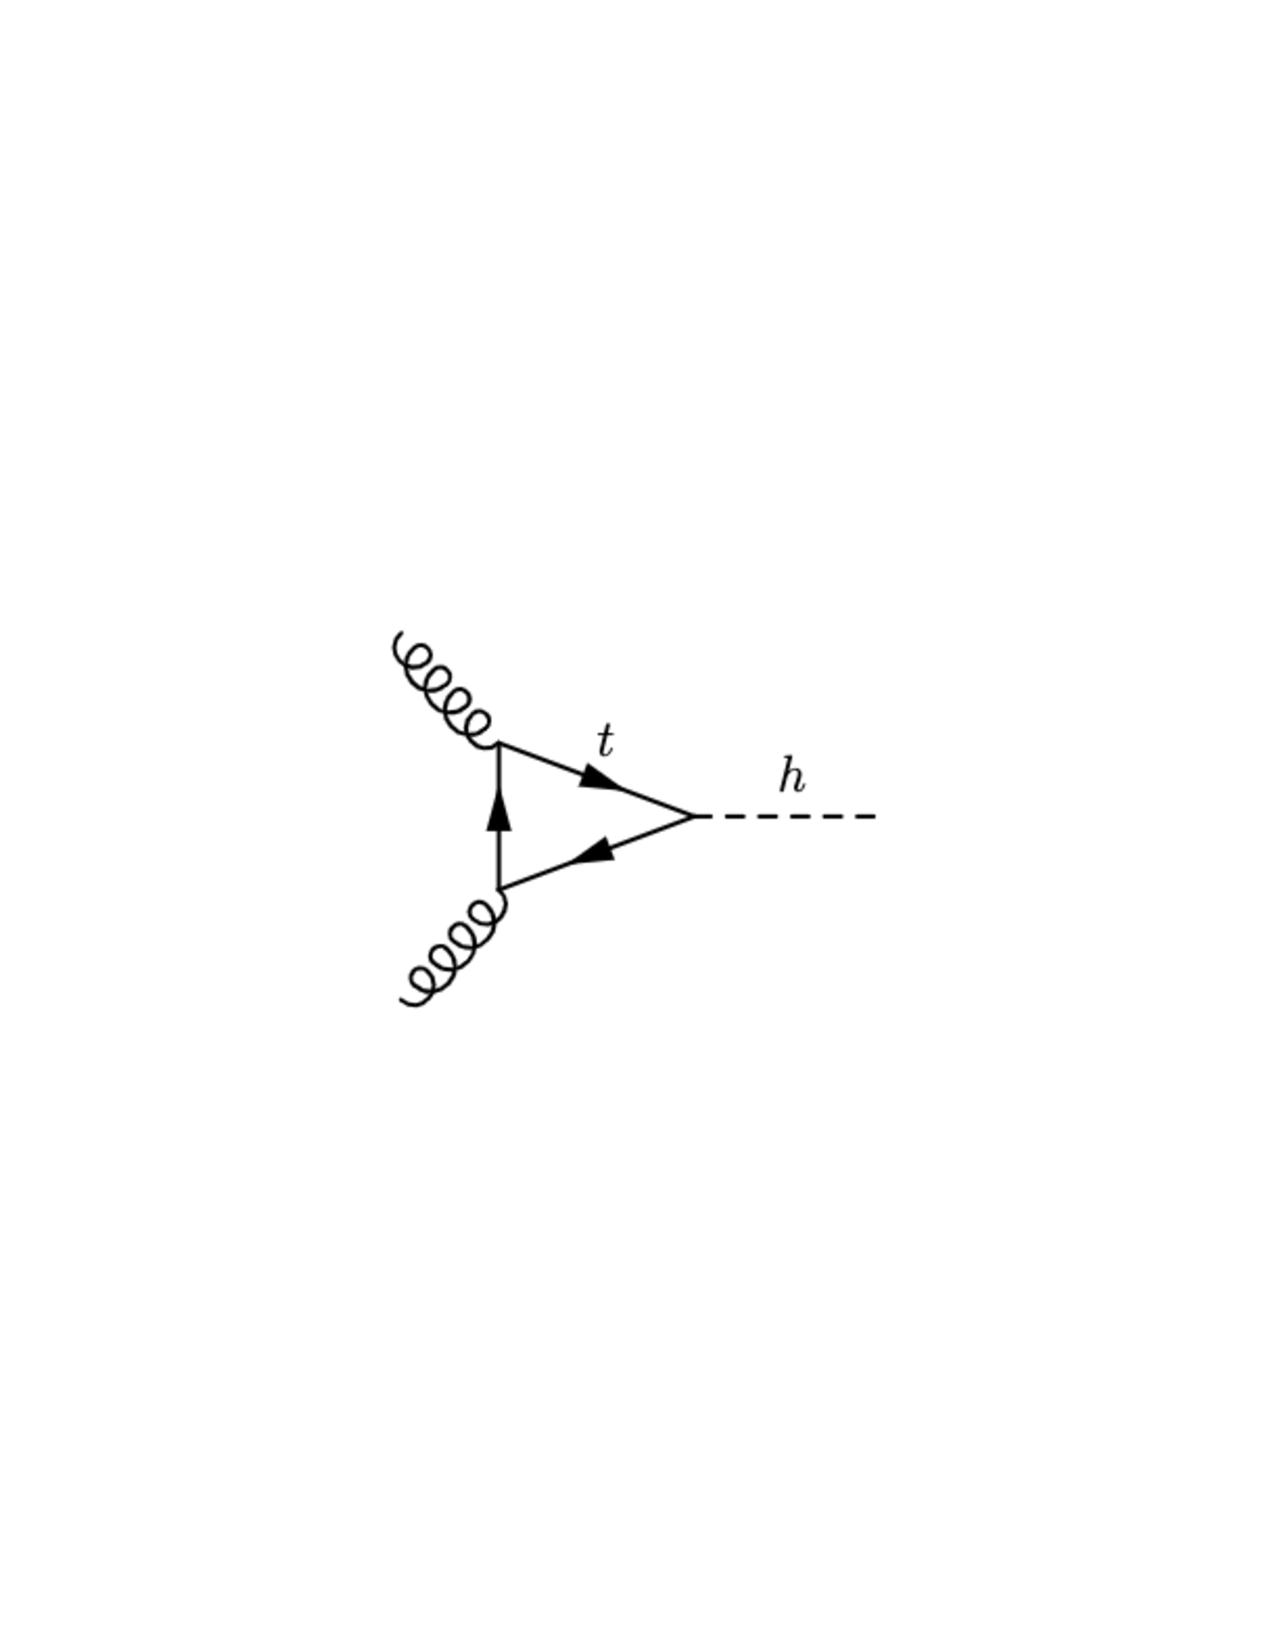
\includegraphics[width = .5\textwidth]{higgs_glue_fusion}
		\caption{Gluon fusion.}
		\label{subfig:higgs_gluon_fusion}
	\end{subfigure}
	~
	\begin{subfigure}[t]{.4\textwidth}
		\centering
		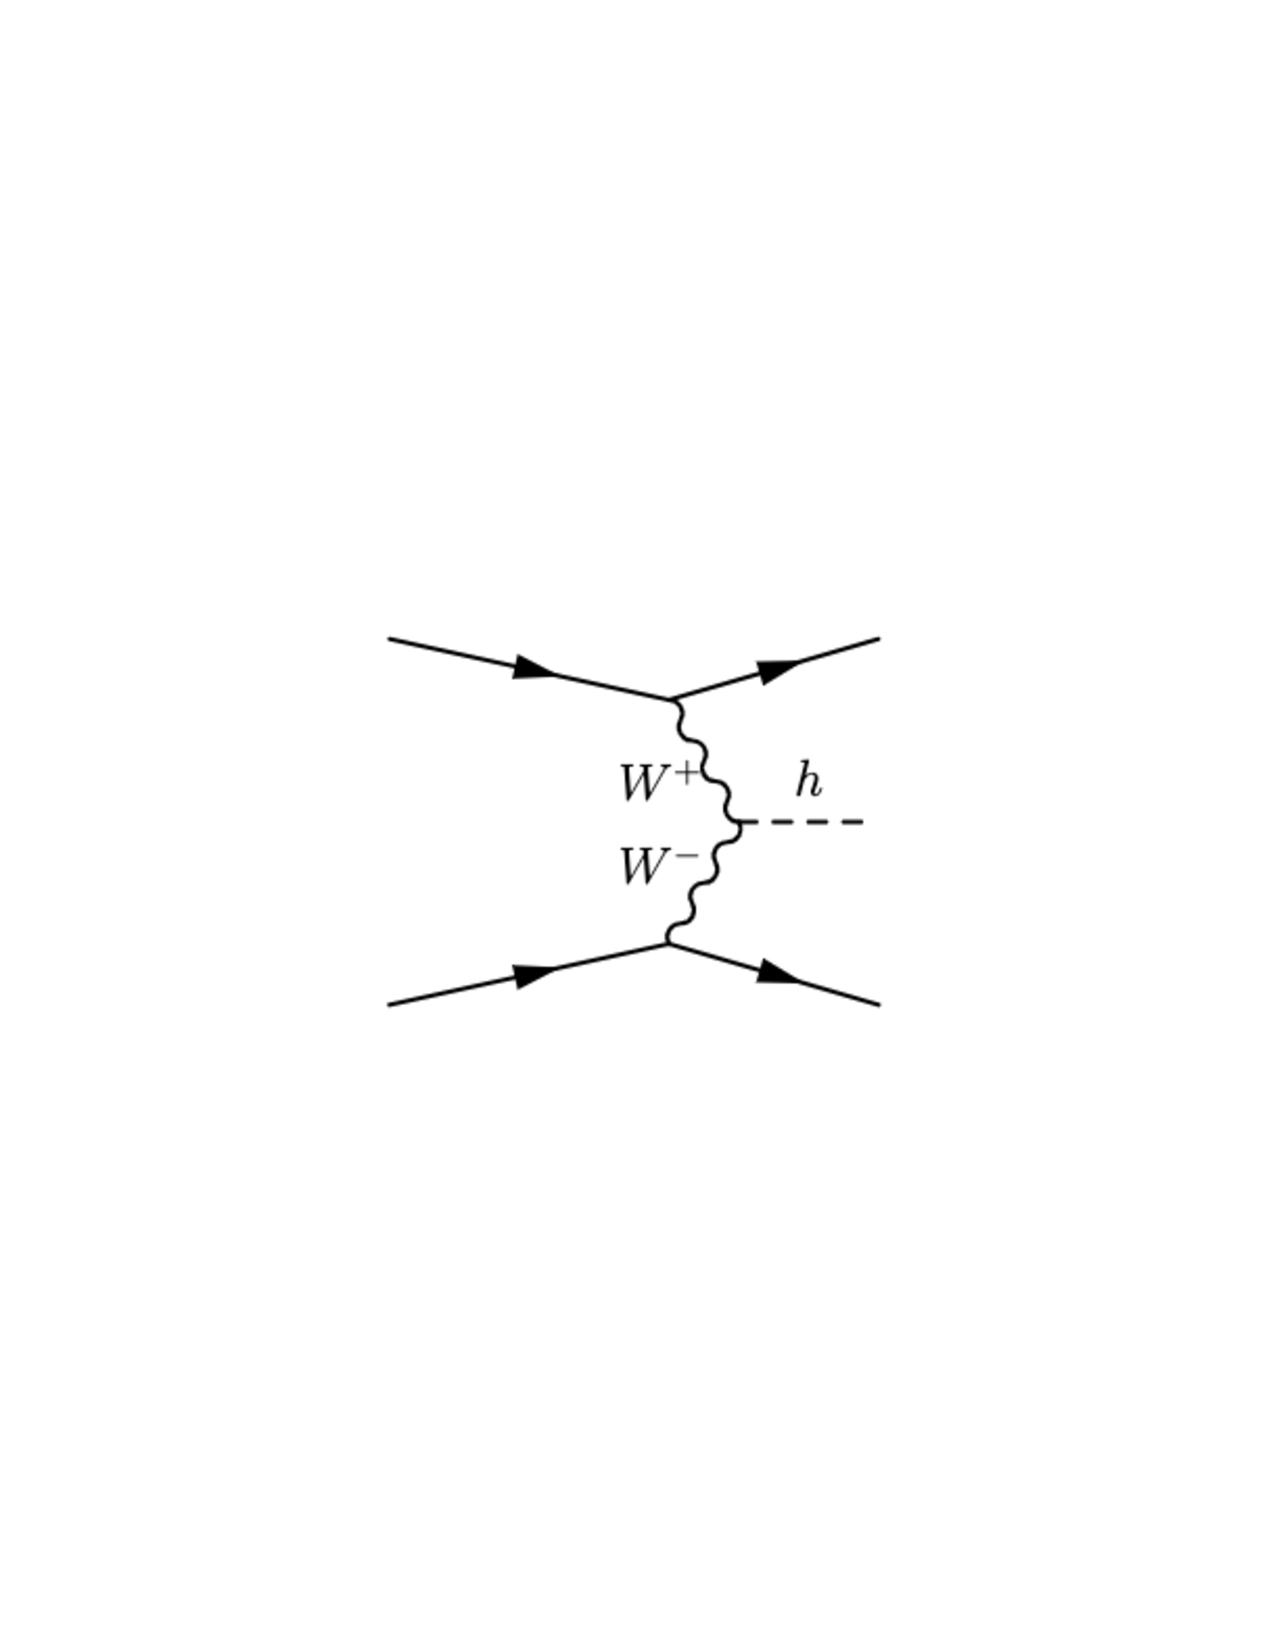
\includegraphics[width = .5\textwidth]{higgs_vector_fusion}
		\caption{Vector boson fusion.}
		\label{subfig:higgs_vector_fusion}
	\end{subfigure}
	\caption{Two largest production channels for the Higgs.~\cite{schwartz}}
\end{figure}
At $S = 13$ TeV, the cross sections for gluon fusion and vector boson fusion are about:
\begin{align}
	\sigma(gg\rightarrow h)\approx 44\;\mathrm{pb} && \sigma(pp\rightarrow qq h)\approx 4\;\mathrm{pb}
	\label{eq:higgs_production_sigma}
\end{align}
so it is obvious that the gluon fusion channel dominates (all other production channels have cross sections of about a picobarn or less). 
The actual Higgs discovery of the Higgs occurred during run 1 of the LHC, when its center of mass energy was only $S = 7$ or $8$ TeV, and 
at this energy these cross sections are about half of what is shown in Eq.~(\ref{eq:higgs_production_sigma}). The vector fusion channel, 
while not as probable as the gluon fusion channel, will contribute mainly along the beam line. Because it is a $t$-channel diagram, this 
cross section will be enhanced when $t$ is small, i.e. when the produced quarks are collinear to the proton frame. At the LHC, this manifests 
itself as two forward jets, and identifying these is one way of determining if the subleading process occurred. 

Now we must discuss decays. There are three \textbf{discovery channels} for the Higgs. We will briefly discuss each of these channels, and 
we will roughly estimate how many times each process occurred during LHC run 1, which was expected to have produced around 500,000 
Higgs bosons through the processes described (and a few more subleading ones). 
\begin{enumerate}
	\item $h\rightarrow ZZ^*\rightarrow 4\ell$, where $\ell$ is any lepton. One of the $Z$ bosons produced in this decay is virtual because 
	$m_H < 2 m_Z$, but nonetheless this is the cleanest decay channel for the Higgs because of the lepton production. Furthermore, the spin 
	of the Higgs can be extrapolated from the angular dependence of the measured leptons. However, the issue with this channel is the low 
	branching ratio: $\mathrm{BR}(h\rightarrow ZZ^*\rightarrow 4\ell)$ is about $10^{-4}$, so out of the 500,000 Higgs produced only about 
	50 decayed through this channel throughout the duration of run 1. Thus although this channel ends up being the cleanest, its low branching 
	ratio made it hard to detect the Higgs here.
	\item $h\rightarrow \gamma\gamma$. This is the channel that you've probably seen a plot of: Higgs decay to two photons through a top loop. 
	This channel's branching ratio is about $\mathrm{BR}(h\rightarrow\gamma\gamma)\approx 0.1\%$, so about 500 of the 
	Higgs decays in run 1 were through the diphoton channel. The reason that this is not the preferred channel is because there is a large amount 
	of QCD background from the process $pp\rightarrow\gamma\gamma$; luckily, this background was not enough to stop the ATLAS 
	Collaboration.
	\item $h\rightarrow WW^*\rightarrow 2\ell 2\nu_\ell$. This channel has a large branching ratio of $\mathrm{BR}(h\rightarrow WW^*
	\rightarrow 2\ell 2\nu_\ell)\approx 1.6\%$, but the two neutrinos in the final state make it hard to reproduce the full kinematics and 
	the process cannot be fully reconstructed because of the invisible neutrinos. 
\end{enumerate}

\begingroup
\begin{wrapfigure}{r}{.4\textwidth}
	\vspace*{-.5cm}
	\centering
	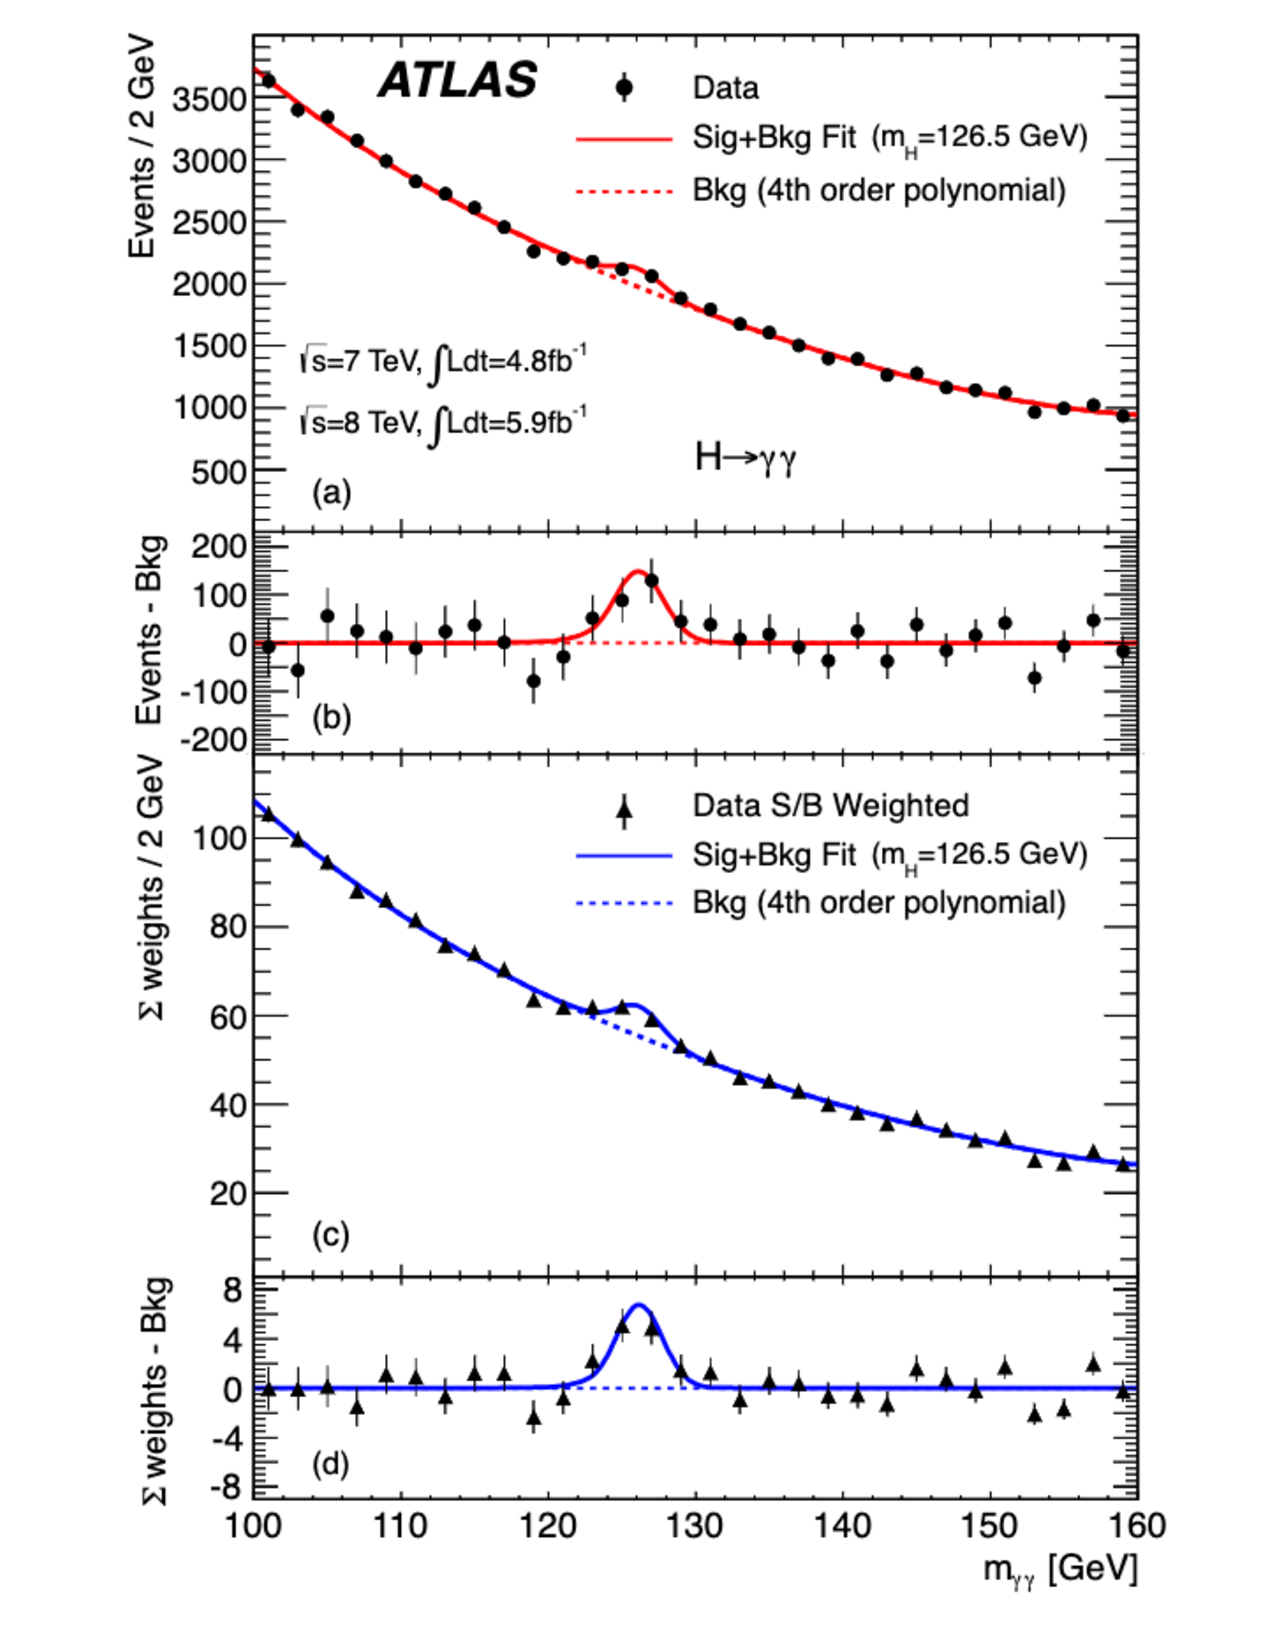
\includegraphics[width = .4\textwidth]{higgs_discovery}
	\caption{Plot released by the ATLAS Collab~\cite{higgs} upon discovery of the Higgs.}
	\label{fig:higgs}
\end{wrapfigure}
The plot showing the discovery of the Higgs boson through the diphoton channel is shown in Figure~\ref{fig:higgs}. There are different weightings 
given to the top and the bottom plot to make the bump more visible. The Higgs decay corresponds 
to the little bump around where the invariant mass $m_\gamma\gamma$ was equal to $m_H \approx 125\;\mathrm{GeV}$; the rest of the 
data is QCD background which is produced from the process $pp\rightarrow\gamma\gamma$ without decaying through the Higgs. 

An important theoretical prediction for this measurement was that of the QCD background for $pp\rightarrow\gamma\gamma$. Because the 
background signal can be shown to be smooth in full QCD, the bump corresponding to the Higgs resonance stands out. If the 
QCD cross section was more irregular, it would be nearly impossible to distinguish the signal from the Higgs. Luckily, nature has decreed 
that the background signal here is smooth. The other two channels do not have this background noise and it is much easier to 
distinguish the Higgs; unfortunately as we discussed, there are other issues in these channels which made the diphoton one the 
smoking gun for the Higgs discovery.

\endgroup

\newpage
\section{Leptons}

\subsection{$e$ and $\mu$ decays}

Leptons are pretty easy-- because they don't hadronize, we don't need any extra bells and whistles like PDFs. Electron-positron colliders like 
LEP can be used to measure simply QED predictions, like $e^- e^+\rightarrow \mu^-\mu^+$, which is like the first process everyone studies 
in QFT. 

If you're thinking about leptonic decay, the easiest thing to do is to think about the leptons in the 4-Fermi theory and see what the 
particles can decay into. This doesn't necessarily work at colliders because it's probable that the collider will be colliding things together at 
an energy which is comparable to the $W$ and $Z$ boson masses, but for decay modes and branching ratios the 4-Fermi theory will do 
the trick. 

Electrons cannot decay because of conservation of charge. They are the lightest charged particles under $U(1)_\mathrm{EM}$ in the 
Standard Model, so they cannot decay into products which are charged and have total mass less than the electron mass. 

However, muons can decay. Since the muon mass is less than the pion mass (the lightest baryon), muons cannot decay to hadrons, and 
so the only decay mode accessible to a muon is $\mu^-\rightarrow\mathrm{leptons}$. This decay will always happen to electrons and 
electron neutrinos because charge must be conserved, and so the following process is the one to compute:
\begin{equation}
	\mu^-\rightarrow\nu_\mu e^-\overline\nu_e
\end{equation}
As we've considered this decay before, I won't discuss it here. Using the 4-Fermi theory, one can show that the decay rate at tree level 
is:
\begin{equation}
	\Gamma_\mu = \frac{G_F^2 m_\mu^5}{192\pi^3}~
	\label{eq:muon_lifetime}
\end{equation}
at tree level, and the scaling as the muon mass to the fifth is necessary by dimensional analysis. The lifetime of the muon, $\tau_\mu = 1 / \Gamma_\mu$, is 
about $2\;\mu\mathrm{s}$ in its rest frame. 

\subsection{$\tau$ decays}

The tau is the most interesting lepton to study for decays because it can decay to hadrons: $m_\tau \approx 2$ GeV and $m_\pi\approx 140$ MeV, so 
there will be hadronic decays available to the $\tau$, at least through the pion. We need to estimate what channels it can decay through, and for this 
we actually need a more precise value for the tau mass. The current value is from the PDG:
\begin{equation}
	m_\tau = 1.77686(12)\;\mathrm{GeV}
\end{equation}
Of course, on the exam you won't need this precision, but we might as well work with exact values while we can just pull them from a table. We've already said the 
$\tau$ can decay into pions, but what other particles can it decay to? It can of course decay to other leptons, $\tau\rightarrow \nu_\tau e \nu_e$ or $\tau\rightarrow\nu_\tau 
\mu\nu_\mu$. 

For $\tau$ to decay to other hadrons, it can connect through $W$ exchange to other off diagonal mesons, like $u \overline s$, $c\overline d$, etc. The two decays which 
may be possible which are not CKM suppressed are $\tau^-\rightarrow d \overline u = \pi^-$ (which we've already said is allowed) and $\tau^-\rightarrow s\overline c = 
D_s^-$. Luckily for us, $\tau$ decay to a $D_s$ meson is not kinematically allowed because of the mass of the $D_s$ meson:
\begin{equation}
	m_{D_s} = 1.96834(7) \;\mathrm{GeV}
\end{equation}
This is why we needed a little precision: $m_{D_S}$ is slightly heavier than the $\tau$, so this decay doesn't exist. So, we see the $\tau$ has 3 
\textit{dominant} decay modes:
\begin{align}
	\tau^-\rightarrow \nu_\tau e^-\overline\nu_e && \tau^-\rightarrow \nu_\tau \mu^-\overline\nu_\mu && \tau^-\rightarrow \nu_\tau d \overline u = \nu_\tau \pi^- \pi^0
\end{align}
Note that these are only the most common decay modes which are not CKM suppressed: there are a whole boatload of other hadronic decays the $\tau$ can undergo, 
but these are the most common. 

To estimate the width of the $\tau$, assuming the other particles are massless means we can just replace the $\mu$ mass with the $\tau$ mass in Eq.~(\ref{eq:muon_lifetime}). 
However, the $\tau$ has five decay modes: two leptonic ($e\nu_e\nu_\tau$ and $\mu\nu_e\nu_\mu$) and three hadronic ($\tau^-\rightarrow d\overline u$ with 3 quark colors), 
so there is a multiplicity of 5 that we need to take into account. Performing these changes on our expression for the muon width, we see approximately that:
\begin{equation}
	\Gamma_\tau\approx 5\frac{m_\tau^5}{m_\mu^5}\Gamma_\mu \approx 10^{7}\times \Gamma_\mu
\end{equation}
The lifetime of the $\tau$ is measured to be about $2.9\times 10^{-13}$ seconds, which is consistent with our prediction. The $\tau$ is evidently a very short-lived particle, 
especially when compared to the other leptons. We can also write down the approximate $\tau$ branching ratios, only including the dominant decay modes:
\begin{table}[H]
	\centering
	\begin{tabular}{ | c | c | c | c |}
		\hline
		$\tau$ decay mode & Hadrons & $\nu_\tau e^-\overline\nu_e$ & $\nu_\tau\mu^-\overline\nu_\mu$ \\
		\hline
		Approximate branching ratio & 60\% & 20\% & 20\% \\
		\hline
	\end{tabular}
	\caption{Dominant decay modes of the $\tau$ lepton.}
	\label{table:tau_decay}
\end{table}
When other hadronic modes are taken into account (including CKM-suppressed modes) the branching ratio becomes more complicated and the branching ratio $\mathrm{BR}(\tau^-
\rightarrow\nu_\tau\ell\overline\nu_\ell)\approx 17\%$. The actual branching ratio for $\tau^-\rightarrow\pi^-\pi^0\nu_\tau$ is only about 26\% once everything is said in done; however, 
the total hadronic branching ratio $\mathrm{BR}(\tau^-\rightarrow\mathrm{hadrons})\approx 65\%$\footnote{I'm not sure why the entire 
hadronic rate is close to what we approximated although the specific process that we estimated is not close at all to its rate; I'd expect 
$\mathrm{BR}(\tau\rightarrow\nu_\tau\ell\overline\nu_\ell) / \mathrm{BR}(\tau\rightarrow\mathrm{hadrons})\approx 1 / 3$, but in reality it 
equals $17 / 26$.}.

\newpage
\section{Hadrons: The Particle Zoo}

The quark sector of the SM is harder to analyze at colliders than the lepton sector because of confinement: quarks can only be found in 
nature in colorless combinations, so decay rates and modes will inevitably involve integrals over quark PDFs. 

Let's briefly discuss some common hadrons to know. We already know where the pseudoscalar nonet comes from: this includes the pions, 
kaons, $\eta$, and $\eta'$ (although the $\eta'$ is not a pseudo-Goldstone boson). Other common mesons are \textbf{D mesons}, which are 
combinations of a charm quark with another antiquark, $c\overline q$, and \textbf{B mesons}, which are formed from a bottom quark and 
another antiquark, $b\overline q$

\subsection{Light quarks}

cHiRaL pErTuRbAtIoN tHeOrY

% Pion decays: pi^\pm\rightarrow vs \pi^0 -> \gamma\gamma

\subsection{Charm / bottom quarks}

The bottom quark forms \textbf{B mesons} and the charm quark forms \textbf{D mesons}. The most common hadrons formed with $b$ 
or $c$ quarks are:
\begin{align}
	B^- = b\overline u && B^0 = b\overline d && B_s^0 = b\overline s \\
	D^+ = c\overline d && D^0 = c\overline u && D_s^+ = c\overline s
\end{align}
$b$ and $c$ quarks also form \textbf{bottomonium} and \textbf{charmonium}. I didn't have time to read up on quarkonium, but it's an 
interesting topic that's worth discussing during another session.

Let's start by thinking about the decay modes for $b$ quarks; even though they are in different generations, the physics of the $b$ and $c$ 
quarks are roughly the same. The $b$ decays primarily through the weak interaction via exchange of a $W^-$. The dominant coupling would 
be the one which is not CKM suppressed, but the $t$ is HUGE so the $b$ quark can't decay into a top. Examining the Wolfenstein 
parameterization, we see that $V_{cb} = \lambda^2$ but $V_{ub} = \lambda^3$, so the dominant decay mode is $b\rightarrow W^- c$. 
This means that \textit{B mesons primarily decay into D mesons and $W$ decay products}, since the $W$ is a virtual particle which 
must decay into other decay products.

To estimate the lifetime of a $B$ meson, we need to determine the number of channels it can fully decay into. Since each channel will 
differ from what the $W$ boson decays into, we need to take a look at the mesons which can be formed from $W$ decay. The approximate 
mass of $B$ mesons is around 5.2 GeV. These mesons which can be created from $W$ decay which are not CKM suppressed are 
$\pi^- = d\overline u$ and $D_s^- = s\overline c$. These have masses:
\begin{align}
	m_{D}\approx 1.8\;\mathrm{GeV} && m_\pi\approx 140\;\mathrm{MeV}
\end{align}
Since the $B$ decays into a $D$ and a $W$ product, there is $m_B - m_D\approx 3.4\;\mathrm{GeV}$ of energy left for the $W$ to have. 
This means it can primarily decay leptonically into any lepton-neutrino pair, or hadronically into either into a $D$ or a $\pi$; each of these 
hadronic decay modes has 3 channels, one for each color. Thus there are 9 possible channels for the decay; in the limit where $m_b$ is 
the only mass we care about\footnote{I would have thought that we would use the $B$ meson mass here, not the $b$ quark mass. However, this is what Schwartz's notes have, so we'll use this for now.}:
\begin{equation}
	\Gamma_B\approx 9 |V_{cb}|^2\frac{m_b^5}{m_\mu^5} \Gamma_\mu\approx 10^{-6} \;\Gamma_\mu
\end{equation}
which means $B$ mesons decay on the order of $\tau_B = 10^{-12}$ seconds in their rest frame. 

In this time in their rest frame, $B$ mesons travel on the order of $c\tau_B \approx 0.5$ mm before decaying. This is further amplified by the 
effects of time dilation: a particle moving relativistically typically has a $\gamma$ factor of 10 or more, so we would expect the $B$ meson 
to travel about $5$ millimeters in the lab frame before decaying. Since the spatial resolution of detectors is on the order of tens or 
hundreds of micrometers, they are usually able to resolve $B$ meson tracks before they decay. An indicator of $B$ meson decay is 
a large number of charged particles being found in the final state, since both the produced $D$ meson and the $W^*$ will decay into 
particles, which are often charged. For example, a common decay of the $B^0$ meson is:
\begin{equation}
	B^0\rightarrow (D^+\rightarrow (K^+\rightarrow\pi^+\pi^0) \pi^+\pi^-)\mu^-\overline \nu_\mu
\end{equation}

Charm quark decays have very similar physics to $b$ quark decays, just their decays are less involved (since a B meson usually 
decays to a D meson!). The non-CKM suppressed channel is $c\rightarrow W^+ s$, which means $D\rightarrow K W^*$, and 
the virtual $W$ then decays further into a final state with energy less than $m_D - m_K \approx 1.3\;\mathrm{GeV}$ (the mass of the 
kaon is about $500$ MeV). This gives two leptonic decay states, $W^*\rightarrow e\nu_e$ and $W^*\rightarrow \mu\nu_\mu$, and 
the only CKM-favored hadronic decay is $W^*\rightarrow u\overline d$, hence there are 5 order 1 decay channels. So, we estimate that:
\begin{equation}
	\Gamma_D\approx 5 |V_{cs}|^2 \frac{m_c^5}{m_\mu^5} \Gamma_\mu\approx 10^{-6}\;\Gamma_\mu
\end{equation}
which is the same order as $B$ meson decays, on the order of picoseconds. When this calculation is done fully, it turns out that 
the decay length for a $D$ meson is about 300 $\mu$m, which is actually shorter than the $B$ meson, despite the $D$ being 
lighter and in an earlier generation than the $B$.

\subsection{Top quarks}

As the heaviest particle in the Standard Model, the top has a relatively unique place in the theory when talking about decays. Current 
measurements of the top mass and width give us:
\begin{align}
	m_t = 172.9(4) \;\mathrm{GeV} && \Gamma_t = 1.42^{+0.19}_{-0.15} \;\mathrm{GeV}
\end{align}
Note that the top mass has a relatively large uncertainty when compared to other SM particle; it is hard to study the top because it decays so 
fast. The lifetime of the top is $\tau_t = (\Gamma_t)^{-1} \times (6.58\times 10^{-25} \mathrm{GeV}\cdot\mathrm{s})\approx 5\times 
10^{-24} \;\mathrm{s}$. In practice, this lifetime is so short that the $t$ quark does not hadronize; the other heavy quarks like the charm and 
strange have lifetimes on the order of $10^{-12}$ and $10^{-13}$, so they do not have this problem.

% Production of the top quark: gluon gluon fusion
At colliders, the top is produced primarily through gluon or quark fusion, $gg\rightarrow t\overline t$ or $q\overline q\rightarrow t\overline t$. 
The first discovery of the top was made at the Tevatron (a $p\overline p$ collider) in 1995 (about $85\%$ of the tops produced here were 
from quark annihilation). This didn't come as a surprise, as the existence of the top was required for anomaly cancellation in the Standard 
Model, so physicists knew they were looking for another quark: they just didn't know exactly where to look until the discovery. 

Top decay primarily happens through the weak interaction. More than 99\% of the time, the top decays as
\begin{equation}
	t\rightarrow b W^+\rightarrow b (\textnormal{W decay products}).
\end{equation}
The other $< 1\%$ of decays are primarily $t\rightarrow d W^+$ or $t\rightarrow s W^+$, but they are CKM suppressed from the $t\rightarrow 
b W^+$ weak decays. Note that this is the only quark that can decay into a \textit{real} $W$ boson, as opposed to a virtual $W$ boson, since 
$m_t > m_W$. The top has a branching ratio into these final states of:
\begin{table}[H]
	\centering
	\begin{tabular}{ | c | c | c | c | c | }
		\hline
		$t$ decay mode & $q\overline q b$ & $e^+\nu_e b$ & $\mu^+\nu_\mu b$ & $\tau^+ \nu_\tau b$ \\
		\hline
		Approximate branching ratio & 66.5\% & 13.3\% & 13.4\% & 7.1\% \\
		\hline
	\end{tabular}
	\caption{Dominant decay modes of the $t$ quark.}
	\label{table:t_decay}
\end{table}
At colliders when a top-antitop pair is created, there are three possible types of final states. The decay can be \textbf{hadronic}, where 
both tops decay to hadrons; \textbf{leptonic}, where both tops decay to hadrons; and \textbf{semi-leptonic}, where one top decays to 
hadrons and one top decays to leptons. We've seen that leptonic channels tend to be the easiest ones to use at colliders to get the 
cleanest signals, since they have the least amount of background and one doesn't have to worry about hadronization. However, 
top decays are usually studied \textit{semi-leptonically}; fully leptonic decays make it hard to reconstruct the full kinematics of the experiment 
since they have two final state neutrinos which are not picked up by the detector. 

% Final decay products: semileptonic ones are easiest to measure because there's only one invisible particle (the $\nu$). 

\subsection{Strong coupling measurements}

TODO

\newpage
\section*{Appendix A: Formulas}

\begin{itemize}

	\item Masses of Standard Model particles:
	\begin{table}[H]
	\centering
	\begin{tabular}{ | c | c | c | c | c | c | c | c | }
		\hline
		$\nu$ & e & u & d & s & $\mu$ & $\pi^0$ & $\pi^\pm$ \\
		\hline
		$\approx 0$ & 0.511 MeV & 2.2 MeV & 4.7 MeV & 93 MeV & 110 MeV & 134 MeV & 139 MeV \\
		\hline
		\end{tabular}
		\begin{tabular}{ | c | c | c | c | c | c | c | c | c | }
		\hline
		$p^+$ & $n^0$ & c & $\tau$ & b & W & Z & H & t \\
		\hline
		938 MeV & 939 MeV & 1.3 GeV & 1.8 GeV & 4.7 GeV & 80 GeV & 91 GeV & 125 GeV & 173 GeV \\
		\hline
	\end{tabular}
	\end{table}
	
	\item Approximate meson masses:
	\begin{table}[H]
	\centering
	\begin{tabular}{ | c | c | c | c | c | }
		\hline
		Meson & $\pi$ & $K$ & $D$ & $B$ \\
		\hline
		Quark content & $u\overline d$ & $s\overline q$ & $c\overline q$ & $b\overline q$ \\
		\hline
		Approximate mass & 140 MeV & 500 MeV & 1.8 GeV & 5.2 GeV \\
		\hline
		\end{tabular}
	\end{table}

	\item Units and the definition of luminosity:
	\begin{align}
		1\;\mathrm{bn} = 10^{-28} \;\mathrm{m}^2 && N = \sigma L_\mathrm{int} && \sigma(pp; \;\mathrm{inclusive})\sim 30 mbn
	\end{align}
	The LHC has a luminosity of $10K$ (low) or $100K$ (high) $pb^{-1} / \mathrm{year}$ and a collision energy of $\sqrt S = 13$ TeV.

	\item Conversion factors ($\Lambda_\mathrm{QCD}\approx 200\;\mathrm{MeV}\approx r_p^{-1}\approx 1 \;\mathrm{fm}^{-1}$):
	\begin{equation}
		1 \;\mathrm{GeV}^{-1} \approx 6.58\times 10^{-25}\;\mathrm{sec}\approx 0.2 \;\mathrm{fm}
	\end{equation}

	\item Decay rate and cross section formulas:
	\begin{align}
		d\Gamma = \frac{1}{2 M} \overline{|\mathcal M|^2} d\Pi_\mathrm{LIPS} && d\sigma = \frac{1}{4 E_1 E_2 |\vec v_1 - \vec v_2|}\,
		\overline{|\mathcal M|^2}\,d\Pi_\mathrm{LIPS}
		\\
		 \tau = \frac{1}{\Gamma} && \textnormal{decay length} = \gamma c\tau
	\end{align}
	where $E_1$ and $E_2$ ($v_1$ and $v_2$) are the energies (velocities) of the incoming particles in the frame you are working in. 
	For two body decay / scattering in the CoM frame:
	\begin{align}
	d\sigma = \frac{1}{64\pi^2 s}\sqrt{1 - \frac{4 m_f^2}{s}} \;\overline{|\mathcal M|^2} d\Omega && (\textnormal{Massless initial, equal mass 
	final}) 
	\end{align}
	
	\item Loop factors: Loops are typically suppressed by an order of about:
	\begin{equation}
		\frac{1}{16\pi^2} = 0.006\approx \frac{1}{100}
	\end{equation}
	times the coupling squared. This comes from doing the integral out after Wick rotation.
	
	\item Breit-Wigner distribution: Cross section for $s$ channel exchange of particle $A$ exchange after resummation:
	\begin{equation}
		\frac{d\sigma(ff'\rightarrow A\rightarrow \tilde f\tilde f')}{ds}\approx \frac{g^4}{(s - m_A^2)^2 + \Gamma_A^2 m_A^2} \approx \frac{\pi g^4}{\Gamma_A m_A}\delta(s - m_A^2)
	\end{equation}
	
	\item Value of SM couplings (all couplings are measured at scale $\mu_{\overline{MS}} = m_Z$):
	\begin{align}
		\sin^2\theta_w \sim .2229 && v = 247\;\mathrm{GeV} && \Theta_\mathrm{QCD}\approx 0 \\
		g' = 0.357 && g = 0.652 && g_3 = 1.221 \\
		\alpha_\mathrm{EM}\approx\frac{1}{129} &&  && \alpha_\mathrm{s} \approx 0.12
	\end{align}
	The Higgs vev $v$ can be measured through computing $G_F$ through muon decay in the 4-Fermi theory.

	\item Electroweak charged and neutral currents:
	\begin{align}
		\mathcal L_\mathrm{EW, int} &= \sum_f \overline\psi_f i\slashed\partial\psi_f + \frac{g}{\sqrt 2} \left( W_\mu^+ j_\mathrm{CC}^{\mu 
		+} + W_\mu^- j_\mathrm{CC}^{\mu -} \right) + \frac{g}{\cos\theta_w} Z_\mu j_\mathrm{NC}^\mu + e A_\mu j_\mathrm{EM}^\mu \\
		&= \sum_f \overline\psi_f i\slashed\partial\psi_f + \frac{e}{\sqrt 2\sin\theta_w} \left( W_\mu^+ j_\mathrm{CC}^{\mu 
		+} + W_\mu^- j_\mathrm{CC}^{\mu -} \right) + \frac{e}{\cos\theta_w\sin\theta_w} Z_\mu j_\mathrm{NC}^\mu + e A_\mu 
		j_\mathrm{EM}^\mu
	\end{align}
	The currents are:
	\begin{align}
	j_{\textnormal{CC}}^{\mu +} &= \overline u^i \gamma^\mu V^{ij}_\mathrm{CKM} P_L d^j +  \overline\nu_e \gamma^\mu P_L e + \overline\nu_\mu \gamma^\mu P_L \mu + \overline\nu_\tau \gamma^\mu P_L \tau \\
	j_{\textnormal{CC}}^{\mu -} &= \overline d^i \gamma^\mu (V_\mathrm{CKM}^\dagger)^{ij} P_L u^j + \overline e \gamma^\mu 
	P_L\nu_e + \overline \mu \gamma^\mu P_L \nu_\mu + \overline\tau \gamma^\mu P_L\nu_\tau = (j_\mathrm{CC}^{\mu +})^\dagger  
	\\
		j_\mathrm{NC}^\mu &= \sum_f \left( \overline\psi_f \gamma^\mu t^3 P_L\psi_f - Q_f\sin^2\theta_w \overline\psi_f\gamma^\mu\psi_f \right) \\
		j_\mathrm{EM}^\mu &= \sum_f Q_f \overline \psi_f \gamma^\mu\psi_f
	\end{align}
	The neutral current is often written in terms of an axial and vector coupling as:
	\begin{equation}
		\mathcal L_\mathrm{NC} = \frac{e}{\sin\theta_w \cos\theta_w} Z_\mu \sum_f \overline\psi_f \left(g_V^{(f)}\gamma^\mu - 
		g_A^{(f)}\gamma^\mu\gamma_5\right) \psi_f
	\end{equation}
	where the couplings are specific to each fermion type and equal:
	\begin{align}
		g_V^{(f)} = \frac{1}{2} t^3_f - Q_f\sin^2\theta_w && g_A^{(f)} = \frac{1}{2} t^3_f
	\end{align}
	
	\item CKM Matrix: Wolfenstein parameterization ($\lambda = \sin\theta_w\approx 0.22$):
	\begin{equation}
	V_\mathrm{CKM} = \begin{pmatrix} 1 - \frac{\lambda^2}{2} & \lambda & \lambda^3 \\
	-\lambda & 1 - \frac{\lambda^2}{2} & \lambda^2 \\
	\lambda^3 & \lambda^2 & 1
	\end{pmatrix}
	\end{equation}
	
	\item 4-Fermi Lagrangian and coupling:
	\begin{equation}
		\mathcal L_\mathrm{4F} = \frac{G_F}{\sqrt 2} j_\mathrm{CC}^{\mu +} j_{\mathrm{CC} \mu}^-
	\end{equation}
	Fermi coupling (note the units):
	\begin{align}
		\frac{G_F}{\sqrt 2} = \frac{g^2}{8m_W^2} = \frac{e^2}{8 m_W^2\sin^2\theta_w} && G_F = 1.16\times 10^{-5}\;\mathrm{GeV}^{-2}
	\end{align}
	
	\item Muon lifetime: This is a good expression to keep in mind because decays from $W$ exchange will be proportional to this, 
	with quark weak interactions being suppressed by the appropriate CKM matrix elements:
	\begin{align}
		\Gamma(\mu^-\rightarrow e^- \overline\nu_e \nu_\mu) = \frac{G_F^2 m_\mu^5}{192\pi^3} && \tau_\mu\approx 2\;\mu\mathrm{s}
		\label{eq:muon_lifetime2}
	\end{align}
	
	\item Flavor-changing weak decay widths: To approximate the width of a particle which decays via the weak interaction, there are a few 
	basic steps:
	\begin{enumerate}
		\item Identify final states. In the case of lepton $\ell$ decay, this will emit a $W^*$ and a neutrino, so the neutrino will be 
		in the final state. In the case of quark $q$ decay, this will emit a $W^*$ (or a real $W$ for the top quark) and quark of the 
		opposite type. The primary decay product will be the one which is not CKM suppressed, which can be read off by the 
		Wolfenstein parameterization (i.e. $s$ quarks will primarily decay to $u W^-$; it would prefer to decay to $c W^-$ from the 
		CKM parameterization
		\item The $W^*$ is virtual and can then decay into either a lepton pair, or a hadron pair, assuming there is enough 
		available energy. This follows the same rules as above: it will decay through any channel which is not CKM suppressed 
		such that it has enough available energy.
		\item If all the particles other than the decaying one are assumed to be massless, the width of the decay is approximately 
		given by taking the muon width $\Gamma_\mu$, Eq.~(\ref{eq:muon_lifetime2}), replacing $m_\mu$ with the 
		mass of the decaying particle, then multiplying by the number of available channels and the appropriate CKM matrix. 
		Remember that meson channels each have multiplicity 3 for color, and lepton channels have multiplicity 1.
	\end{enumerate}

\end{itemize}

\newpage
\section*{Appendix B: Part III Questions}

\begin{itemize}
	\item What is the Higgs mechanism and describe some of the current experimental work searching for the Higgs boson. Discuss the 
	production and decay of the standard model Higgs at the LHC. What are the dominant production mechanisms as a function of the 
	Higgs mass? What are the dominant decay mechanisms, also as a function of the Higgs mass? What are the signatures the 
	experimentalists expect to observe in their apparatus? (Topics, 2006)
	
	\item $e^+ e^-\rightarrow Z^0$ phenomenology. Draw the Feynman diagram. What are the couplings? Draw the cross section as a 
	function of energy. What about $e^+ e^-\rightarrow Z^0 \rightarrow\nu \overline\nu$? This is an invisible process experimentally (can't 
	detect the neutrinos in a collider experiment), but it has been measured. How? Radiative return - running at a higher energy and looking 
	for a single hardphoton with energy $E = \sqrt s - m_Z$. What do these cross-sections look like as a function of energy? (Bob Jaffe, 
	2006)
	
	\item What are the ``typical numerical factors" picked up by fermion loops in Feynman diagrams? (2006)
	
	\item Features of top quark decay. What is the dominant decay of the top quark? What is the experimental signature of production and 
	subsequent decay of a top quark? Why don?t you find any information about mesons like$t\overline u$, $t\overline b$, or $t\overline t$
	in the particle data tables? (Other quarkonium and bound state? What are the sizes of these states? How about $c\overline c$, 
	$b\overline b$ mesons? B, D mesons? Their decays compared to pions? How are they different from each other? OZI rule and 
	quasi-stable states. Strong, EM or weak decays. Pion decays: does $\pi^\pm$ or $\pi^0$ decay faster? (Topics, 2010)
	
	\item Tau decays: branching ratios, write down an expression for the decay width (2010)
	
	\item Estimate the decay rate for the muon, rho, pion, neutron and higgs. (Krishna, 2013)
	
	\item Questions about B-meson decays (dominant decay modes, estimating lifetimes, etc.) Is distance covered by B-meson in lifetime 
	resolvable by the detector? (Will Detmold, 2015)
	
	\item Explain the measurement that led to the discovery of the Higgs particle. What decay channel(s) was (were) studied? What do we 
	know about the various properties of this new particle? What are upcoming measurements going to look for about this particle? (Topics, 
	2018)
	
	\item  Electron positron scattering. He handed a plot with the total scattering as well as the ratio between total scattering and scattering 
	to muon-antimuon. Draw diagrams of processes. Identify particular behaviors on the plot (Bob Jaffe, 2019).
	
\end{itemize}

\newpage
\begin{thebibliography}{99}

\bibitem{pdg}
M. Tanabashi et al. (Particle Data Group), Phys. Rev. D 98, 030001 (2018).

\bibitem{perkins}
D. Perkins. \textit{Introduction to High Energy Physics, 4th edition}. Cambridge University Press (2000).

\bibitem{perelstein}
Perelstein, M. (2010). Introduction to Collider Physics. arXiv 1002.0274.

\bibitem{plehn}
Plehn, T. (2009). Lectures on LHC Physics. arXiv 0910.4182.

\bibitem{schwartz}
Schwartz, M. (2017). TASI Lectures on Collider Physics. arXiv 1709.04533.

\bibitem{ellis}
R. Ellis et al. \textit{QCD and Collider Physics}. Cambridge University Press (1996).

\bibitem{lhc}
https://home.cern/resources/faqs/facts-and-figures-about-lhc

\bibitem{rhic}
https://www.bnl.gov/rhic/physics.asp

\bibitem{w_mass}
Abe, F., \textit{et al}. (1995). Measurement of the W boson mass Physical Review D  52(9), 4784-4827. https://dx.doi.org/10.1103/physrevd.52.4784

\bibitem{higgs}
Collaboration, T. (2012). Observation of a new particle in the search for the Standard Model Higgs boson with the ATLAS detector at the LHC. arXiv 1207.7214.

\bibitem{particle_detectors}
https://home.cern/science/experiments/how-detector-works

\end{thebibliography}

\end{document}